\documentclass[english,11pt]{beamer}

\DeclareMathOperator{\Cov}{Cov}
\DeclareMathOperator{\Var}{Var}
\DeclareMathOperator{\E}{\mathbb{E}}
\DeclareMathOperator{\Proba}{\mathbb{P}}

\newcommand{\Covb}[2]{\ensuremath{\Cov\!\left[#1,#2\right]}}
\newcommand{\Eb}[1]{\ensuremath{\E\!\left[#1\right]}}
\newcommand{\Pb}[1]{\ensuremath{\Proba\!\left[#1\right]}}
\newcommand{\Varb}[1]{\ensuremath{\Var\!\left[#1\right]}}

% norm
\newcommand{\norm}[1]{\| #1 \|}

\newcommand{\indep}{\rotatebox[origin=c]{90}{$\models$}}





\usepackage{mathptmx,amsmath,amssymb,graphicx,bibentry,bbm,babel,ragged2e}

\makeatletter

\newcommand{\noun}[1]{\textsc{#1}}
\newcommand{\jitem}[1]{\item \begin{justify} #1 \end{justify} \vfill{}}
\newcommand{\sframe}[2]{\frame{\frametitle{#1} #2}}

\newenvironment{centercolumns}{\begin{columns}[c]}{\end{columns}}
%\newenvironment{jitem}{\begin{justify}\begin{itemize}}{\end{itemize}\end{justify}}

\usetheme{Warsaw}
\setbeamertemplate{footline}[text line]{}
\setbeamertemplate{headline}{}
\setbeamercolor{structure}{fg=purple!50!blue, bg=purple!50!blue}

\setbeamersize{text margin left=15pt,text margin right=15pt}

\setbeamercovered{transparent}


\@ifundefined{showcaptionsetup}{}{%
 \PassOptionsToPackage{caption=false}{subfig}}
\usepackage{subfig}

\usepackage[utf8]{inputenc}
\usepackage[T1]{fontenc}

\usepackage{multirow}

\usepackage{mdframed}


\makeatother

\begin{document}




% Des jumeaux à la famille élargie : intégration et validation des modèles de simulation
\title{From digital twins to their extended family: integration and validation of simulation models}

\author{J.~Raimbault$^{1,2,3,4}$\\
\texttt{juste.raimbault@ign.fr}
}


\institute{$^{1}$LASTIG, Univ. Gustave Eiffel, IGN-ENSG\\
$^{2}$CASA, UCL\\
$^{3}$UPS CNRS 3611 ISC-PIF\\
$^{4}$UMR CNRS 8504 G{\'e}ographie-cit{\'e}s
}


\date{\textit{Journ{\'e}e de la Recherche UGE-IGN-ENSG 2023}\\
30/03/2023
}

\frame{\maketitle}


\section{Introduction}


% Mike - map-territory - modeles 1:1? cf rgs16
% jumeau = processes -> carte d'identite du jumeau seulmt?
% OML: slides OML, spatial SA
% ! dir la: vendre OML - coeur du jumeau, compare dafni ; call intrapreneur?
% Examples coupling: Sure simplu3d ; ? [quoi depuis ici] -> innovation multiscale
% communs: one slides? [todo ask Alexandra - pres Rchbrune]
% CL: "ca va le jumeau? la famille tout ca"


% Lit jumeaux
% - lien digital twins et complexité:
%Arcaute, Elsa & Barthelemy, Marc & Batty, Michael & Caldarelli, Guido & Gershenson, Carlos & Helbing, Dirk & Moreno, Yamir & Ramasco, Jose Javier & Rozenblat, Céline & Sánchez, Angel. (2021). Future Cities: Why Digital Twins Need to Take Complexity Science on Board.  
%https://www.researchgate.net/publication/354446988_Future_Cities_Why_Digital_Twins_Need_to_Take_Complexity_Science_on_Board/link/6138bca0c76de21e319f536a/download

% - theory/governance:
%Mora, L., Deakin, M., Zhang, X., Batty, M., de Jong, M., Santi, P., & Appio, F. P. (Eds.). (2022). Sustainable Smart City Transitions: Theoretical Foundations, Sociotechnical Assemblage and Governance Mechanisms. Routledge.
%Tout le chapitre est dispo sur google books: https://books.google.fr/books?id=uHxTEAAAQBAJ&lpg=PT8&ots=YBm_fAdvpZ&dq=Sustainable%20Smart%20City%20Transitions%3A%20Theoretical%20Foundations%2C%20Sociotechnical%20Assemblage%20and%20Governance%20Mechanisms&lr&hl=fr&pg=PT14#v=onepage&q&f=false

% - cartographie de la literature:
%Soe, R. M., Schuch de Azambuja, L., Toiskallio, K., Nieminen, M., & Batty, M. (2021). Institutionalising smart city research and innovation: from fuzzy definitions to real-life experiments. Urban Research & Practice, 1-43.pdf en pj

% - real-time GIS data
%Li, W., Batty, M., & Goodchild, M. F. (2020). Real-time GIS for smart cities. International Journal of Geographical Information Science, 34(2), 311-324.pdf en pj

% - urban analytics : policy
%Kandt, J., & Batty, M. (2021). Smart cities, big data and urban policy: Towards urban analytics for the long run. Cities, 109, 102992. pdf en pj

% - link model - real system
%Batty, M. (2019). A map is not the territory, or is it?. Environment and Planning B: Urban Analytics and City Science, 46(4), 599-602. (open access)

% - digital twins
%Batty, M. (2018). Digital twins. Environment and Planning B: Urban Analytics and City Science, 45(5), 817-820.(open access)

% - multimodeling
%Batty, M. (2021). Multiple models. Environment and Planning B: Urban Analytics and City Science, 48(8), 2129-2132. (open access)


\sframe{Digital twins : concepts and reality}{


}


\sframe{Digital twins and Sustainability}{

% si possible carto lit dig twin - sdgs

% Request : "digital twin" AND "sustainable development" (adding "sustainb*" -> too general, include sust economically e.g.)
%   initial corpus?


}



\sframe{OpenMOLE: validation of simulation models}{

% https://hackmd.openmole.org/6yuwyo1dR1aulyqy9iZeyQ#PSE-performances

%     Logiciel libre pour l’exploration et l’évaluation de modèles de simulation   Utilisable avec la majorité des modèles de simulation    Propose une méthodologie d’exploration    Délègue le calcul de manière transparente sur cluster et grille
%     150 000 lignes de code ;   16 000 commits  15 versions  60 contributeurs  Des centaines de modèles explorés  Plusieurs milliards d’heures de calcul

\centering

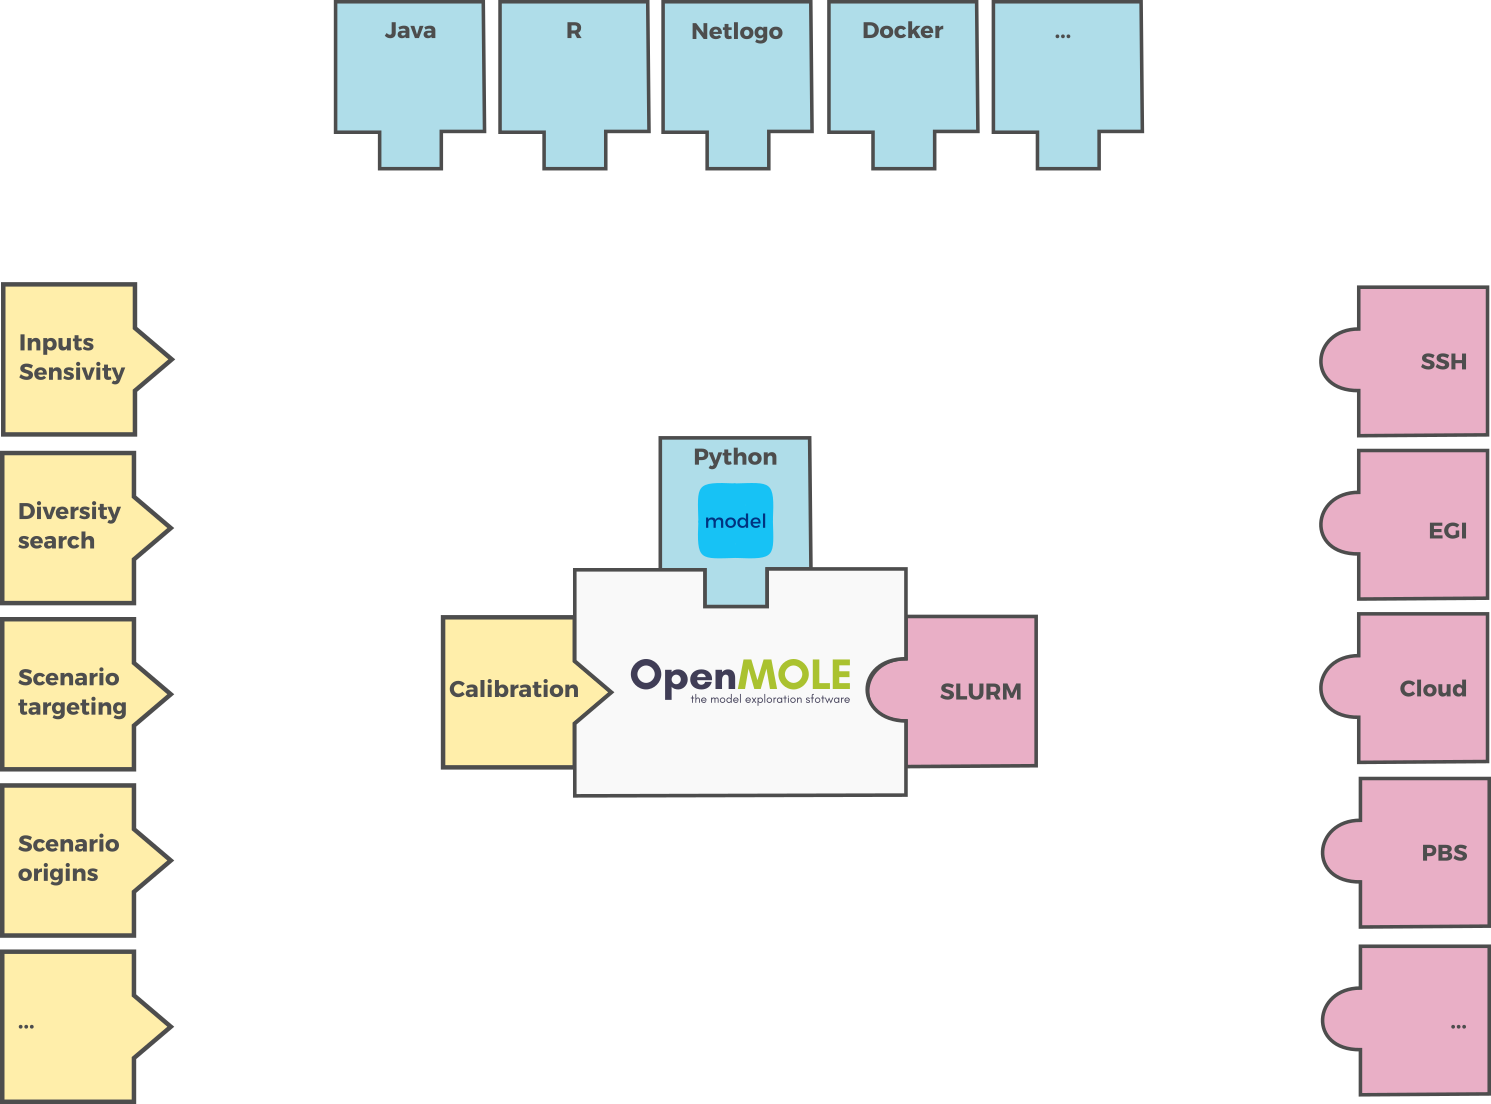
\includegraphics[width=0.9\linewidth]{figures/openmole_axis}

}


\sframe{OpenMOLE: objectively the best}{

% + compare dafni!, mention closed solutions oral

\centering

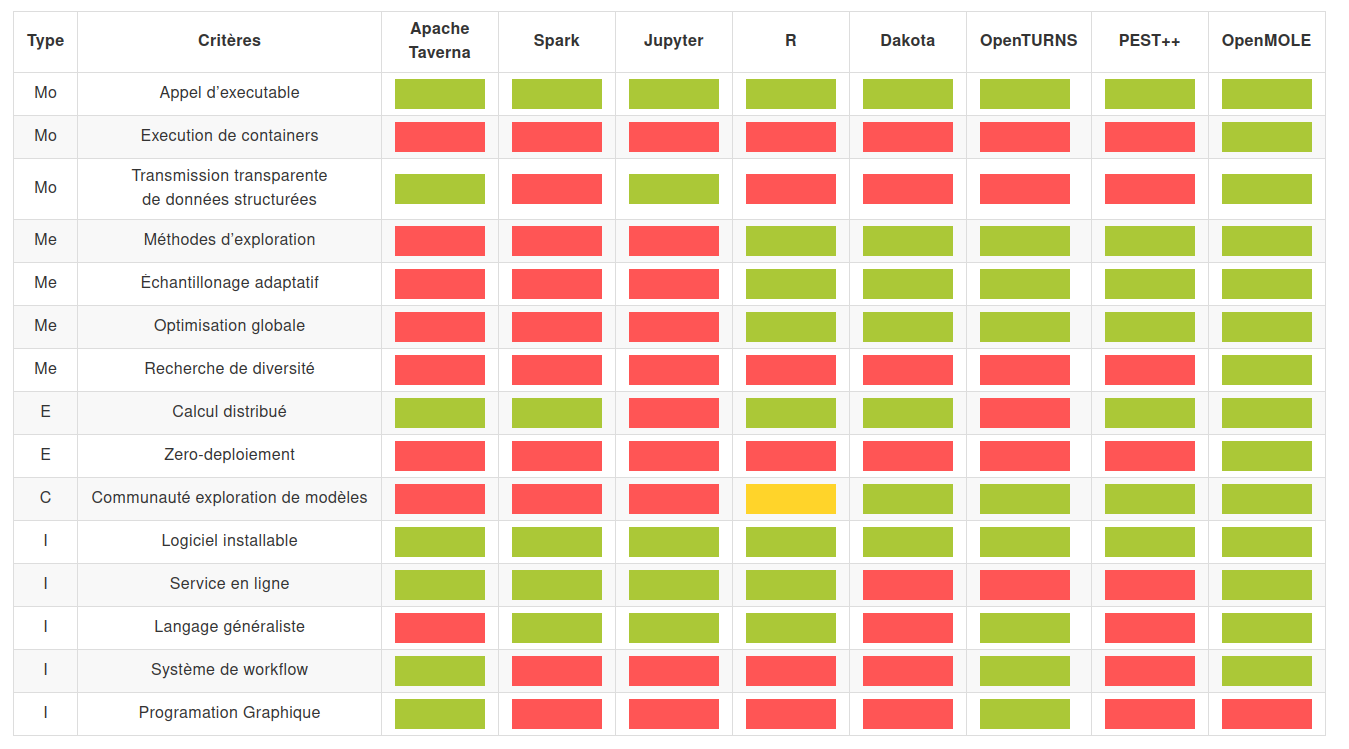
\includegraphics[width=\linewidth]{figures/openmole_benchmark}

}

\sframe{Towards sustainable decision making for territories by integrating and validating simulation models}{

}







\section{Conclusion}


\sframe{Synthesis}{

%\footnotesize

\justify

$\rightarrow$ 

\medskip

$\rightarrow$ 




}




%%%%%%%%%%%%%%%%%%%%%
\begin{frame}[allowframebreaks]
\frametitle{References}
\bibliographystyle{apalike}
\bibliography{biblio}
\end{frame}
%%%%%%%%%%%%%%%%%%%%%%%%%%%%





\end{document}




% CCL

$\rightarrow$ \textbf{Integrated models} capturing complexity of \textbf{urban sustainability} towards \textbf{decision-making}.

\medskip

$\rightarrow$ \textbf{Robust} knowledge from models obtained with the development of \textbf{validation and exploration methods}.

\medskip

$\rightarrow$ \textbf{Applied} knowledge through the construction of \textbf{harmonised databases} upstream and \textbf{transfer methods} downstream.

\medskip

$\rightarrow$ A \textbf{reflexive and interdisciplinary} framework through knowledge mapping.






\sframe{Land-use transport interactions}{


\includegraphics[width=0.39\linewidth]{figures/accessp_withbridge_prd_EN.png}
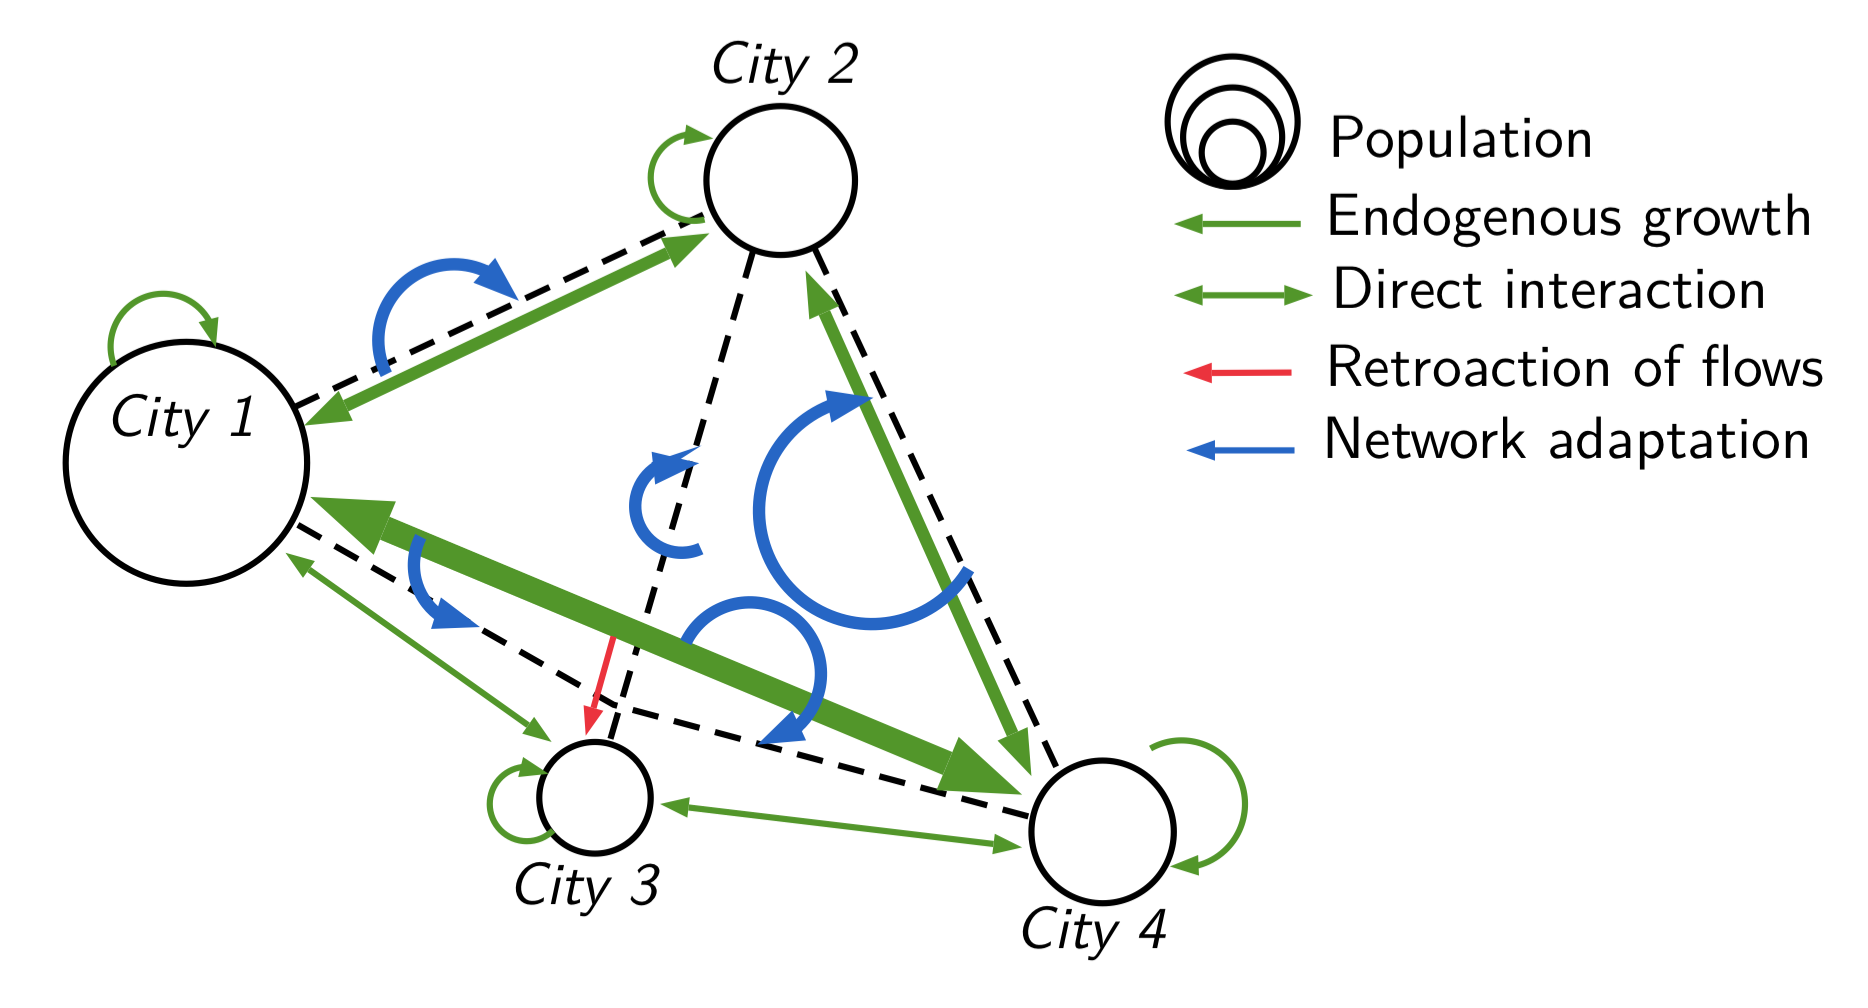
\includegraphics[width=0.6\textwidth]{figures/macrocoevol_en.png}

%\hspace{0.1cm}
%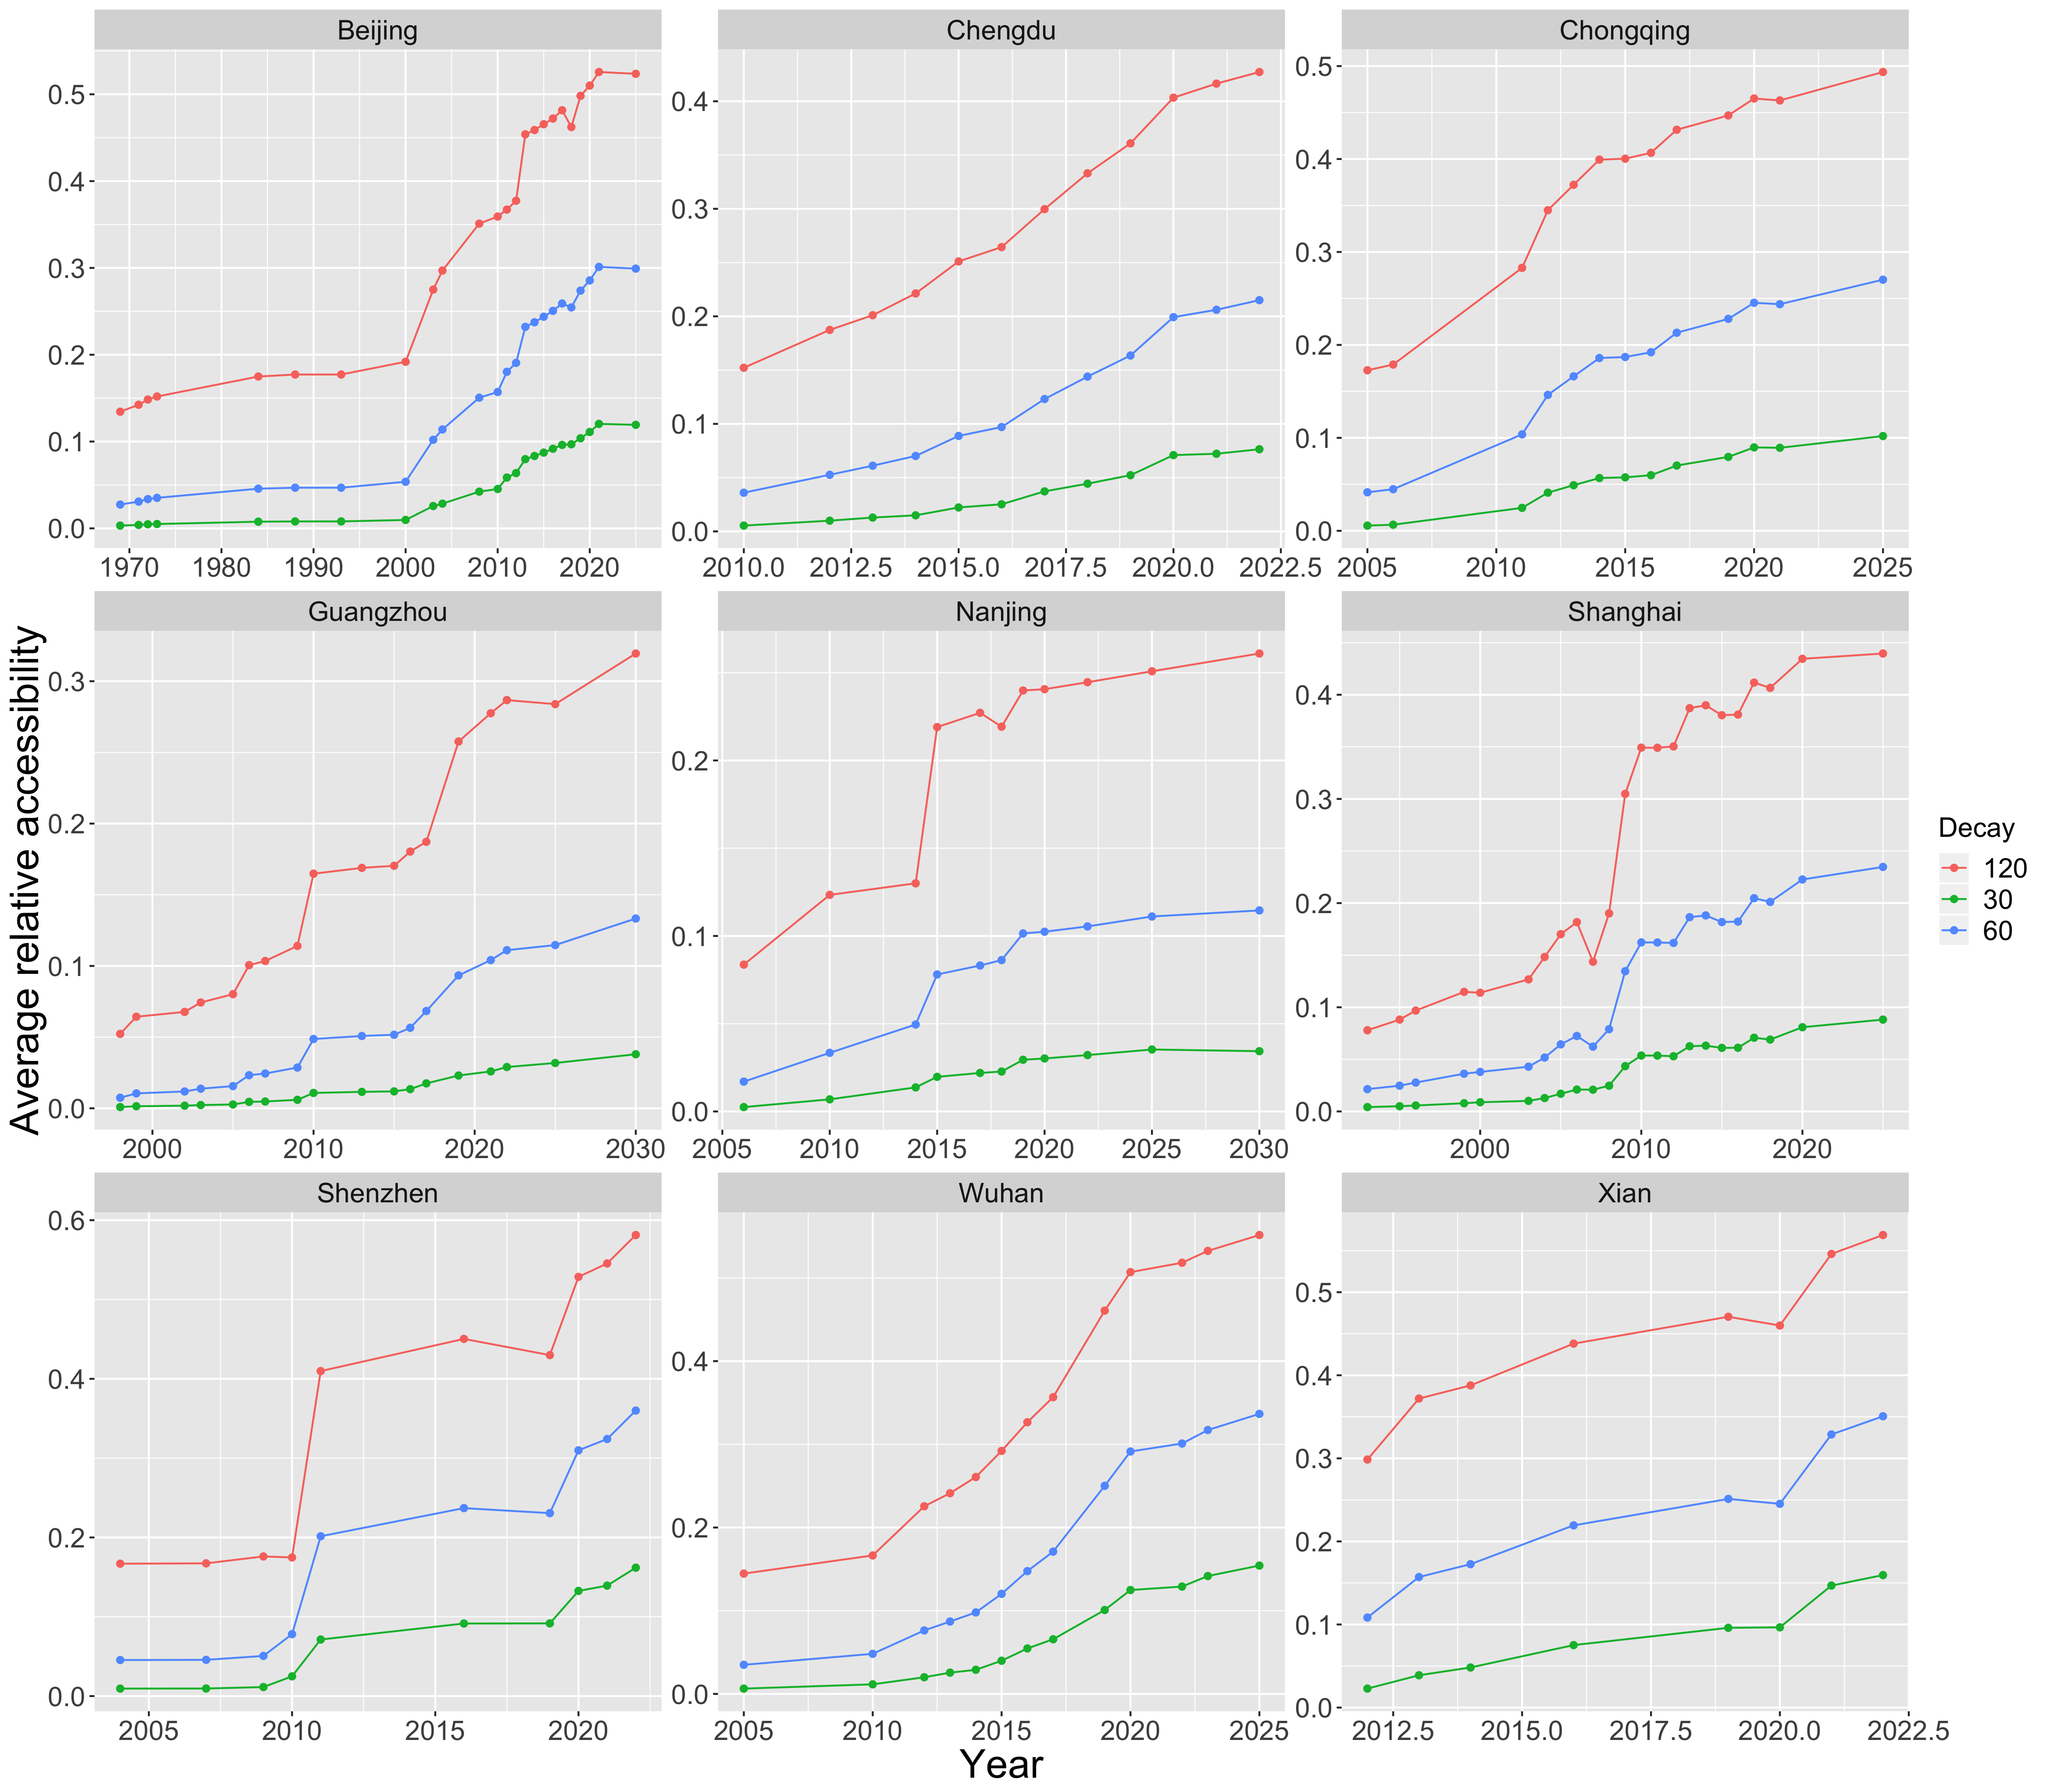
\includegraphics[width=0.52\linewidth]{figures/avgaccess_facet.png}

\medskip


\textit{A modeling approach to the issue of structuring effects of transport infrastructures: co-evolution of networks and territories}

\bigskip

\tiny
%\textcolor{grey}
Raimbault, J. (2019). Evolving accessibility landscapes: mutations of transportation networks in China. In Aveline-Dubach, N., ed. \textit{Pathways of sustainable urban development across China - the cases of Hangzhou, Datong and Zhuhai}, pp 89-108. Imago. ISBN:978-88-94384-71-0

\nocite{raimbault:halshs-02265423}

\smallskip

Raimbault, J. (2020). Indirect evidence of network effects in a system of cities. Environment and Planning B: Urban Analytics and City Science, 47(1), 138-155.

\nocite{raimbault2020indirect}

\smallskip

Raimbault, J. (2021). Modeling the co-evolution of cities and networks. In Handbook of Cities and Networks. Edward Elgar Publishing.

\nocite{raimbault2021modeling}


}


\sframe{Urban morphogenesis}{

\footnotesize


\justify


\begin{center}
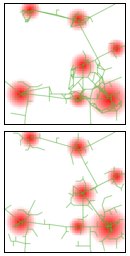
\includegraphics[width=0.25\linewidth,height=0.6\textheight]{figures/meso-nwgrowth.png}
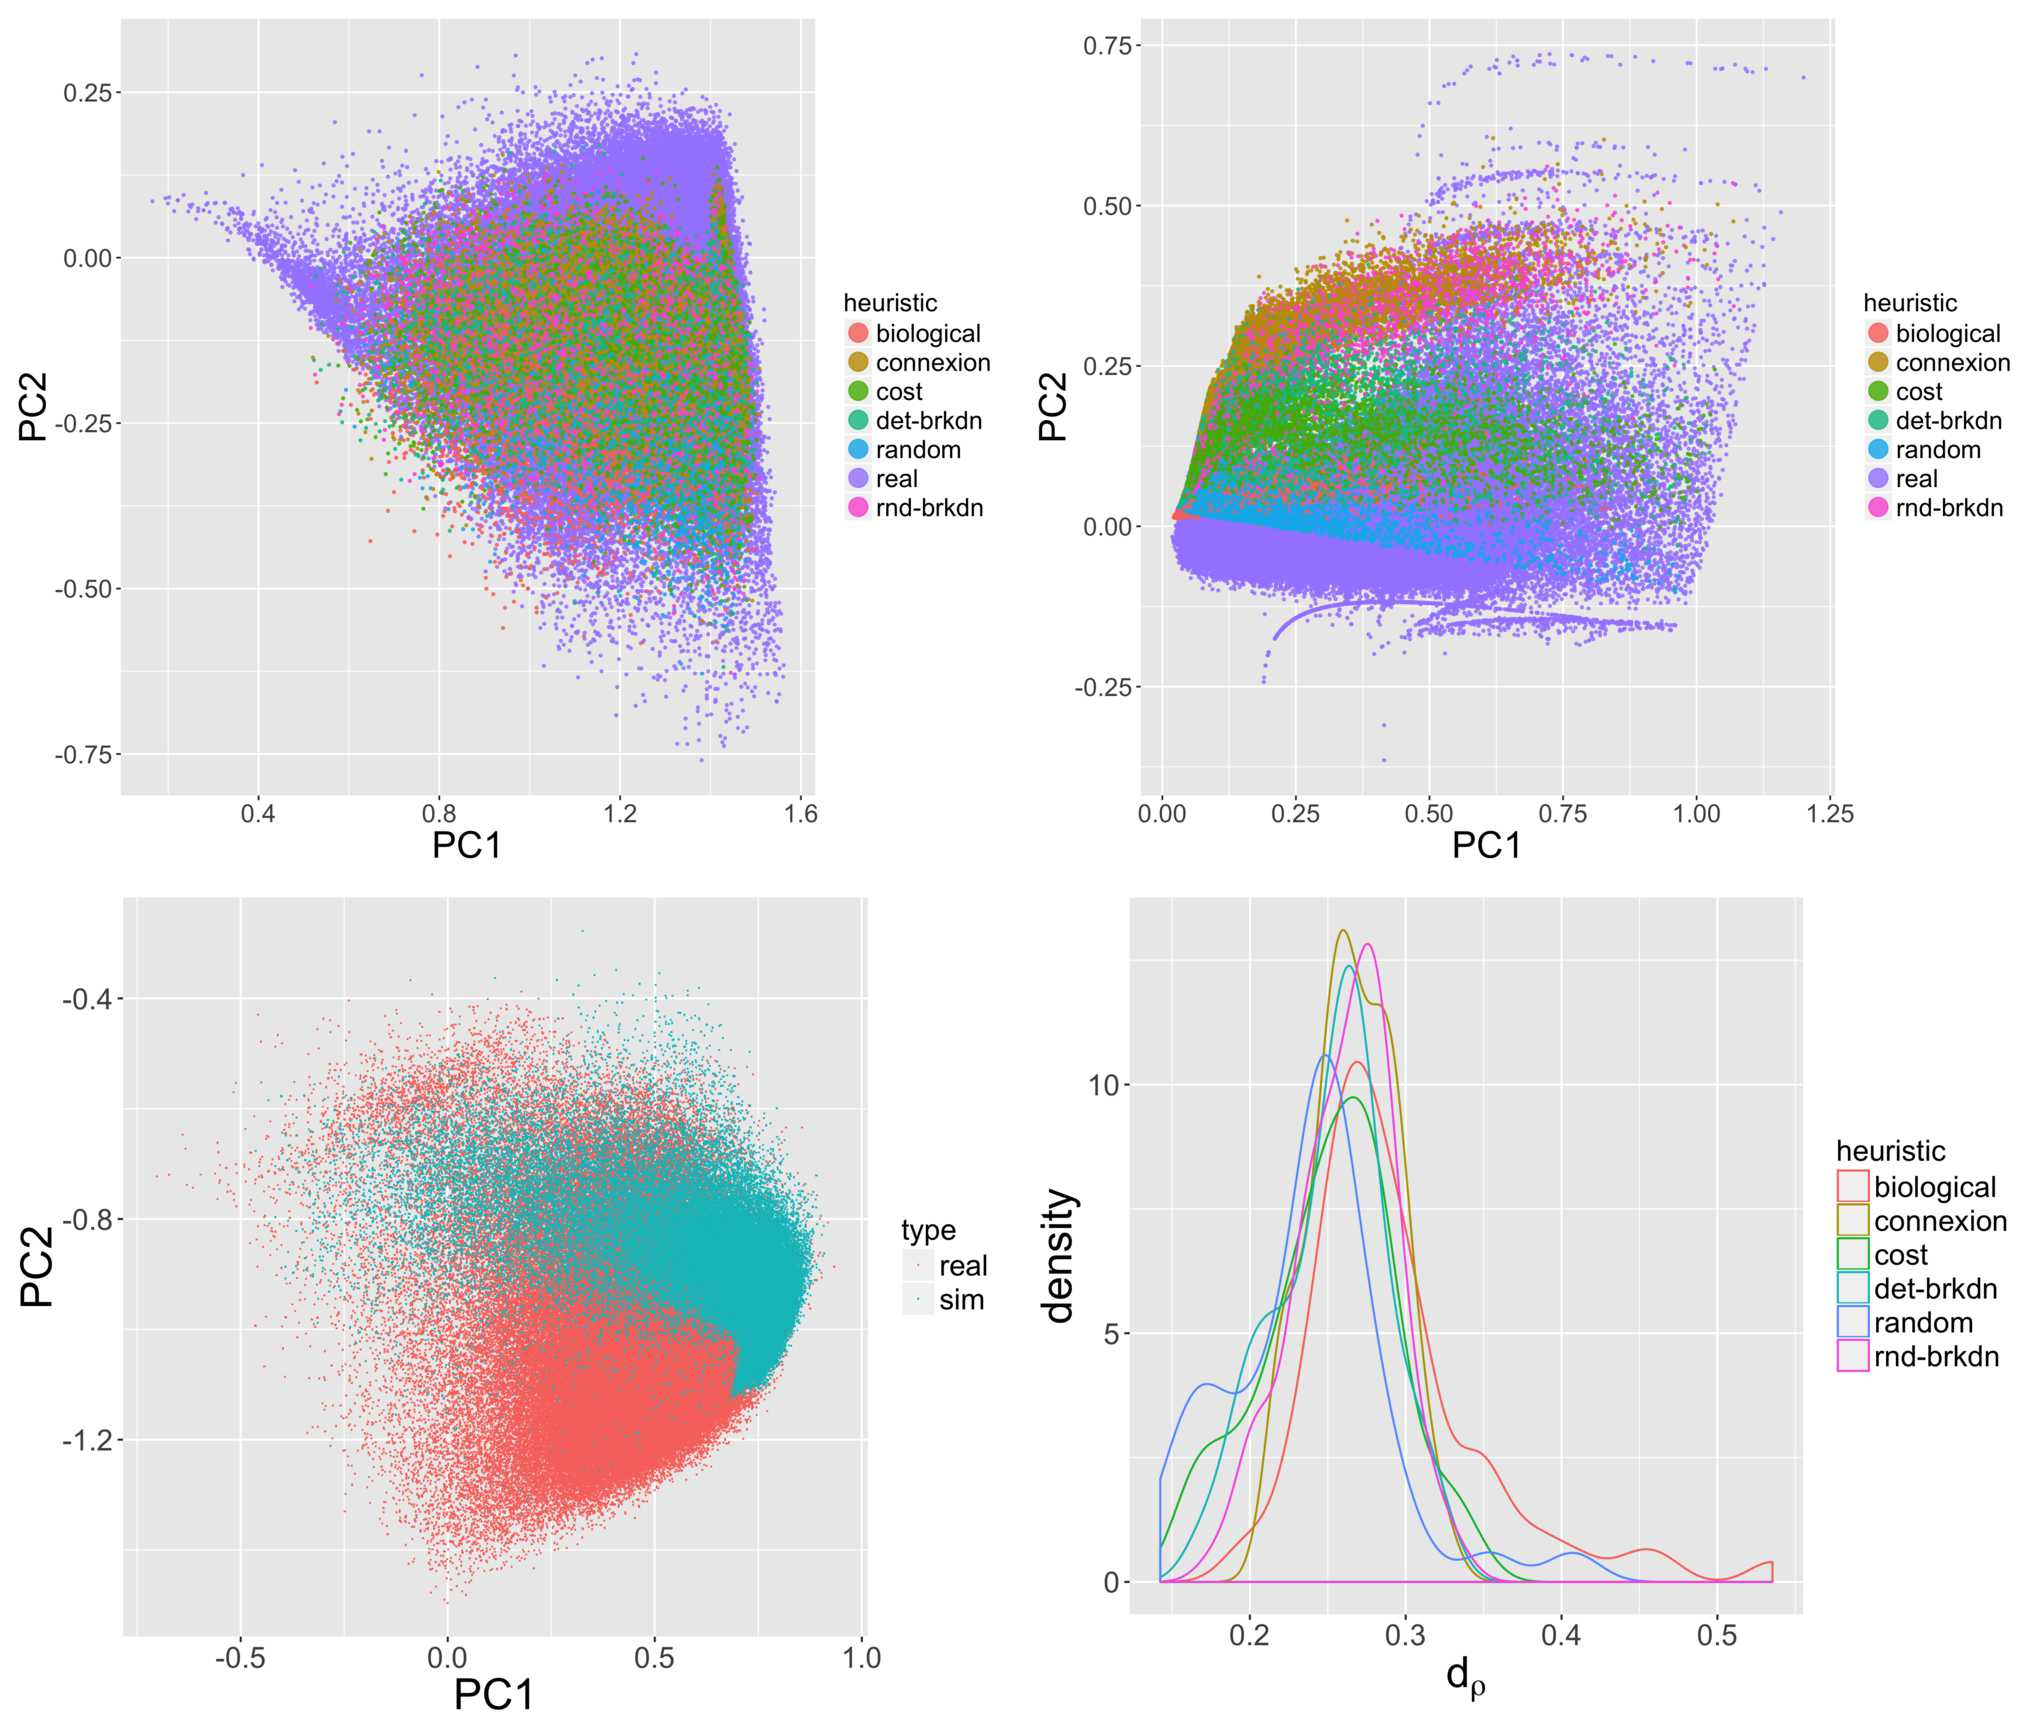
\includegraphics[width=0.6\linewidth,height=0.6\textheight]{figures/meso-calib.jpg}
\end{center}

\medskip

\textit{A morphogenesis model with reaction-diffusion and multi-modeling of network growth: complementarity of heuristics, calibration for Europe on forms and their correlations}


\smallskip

\tiny

Raimbault, J. (2018). Calibration of a density-based model of urban morphogenesis. PloS one, 13(9), e0203516.

\nocite{raimbault2018calibration}

\smallskip

Raimbault, J. (2019). An urban morphogenesis model capturing interactions between networks and territories. In The Mathematics of Urban Morphology (pp. 383-409). Birkhäuser, Cham.

\nocite{raimbault2019urban}

%\smallskip

%Raimbault, J. (2018). Multi-modeling the morphogenesis of transportation networks. In Artificial Life Conference Proceedings (pp. 382-383).
}




\sframe{Urban systems and sustainability}{


%Syst{\`e}mes de villes / Gouvernance

% circular economy

\begin{center}
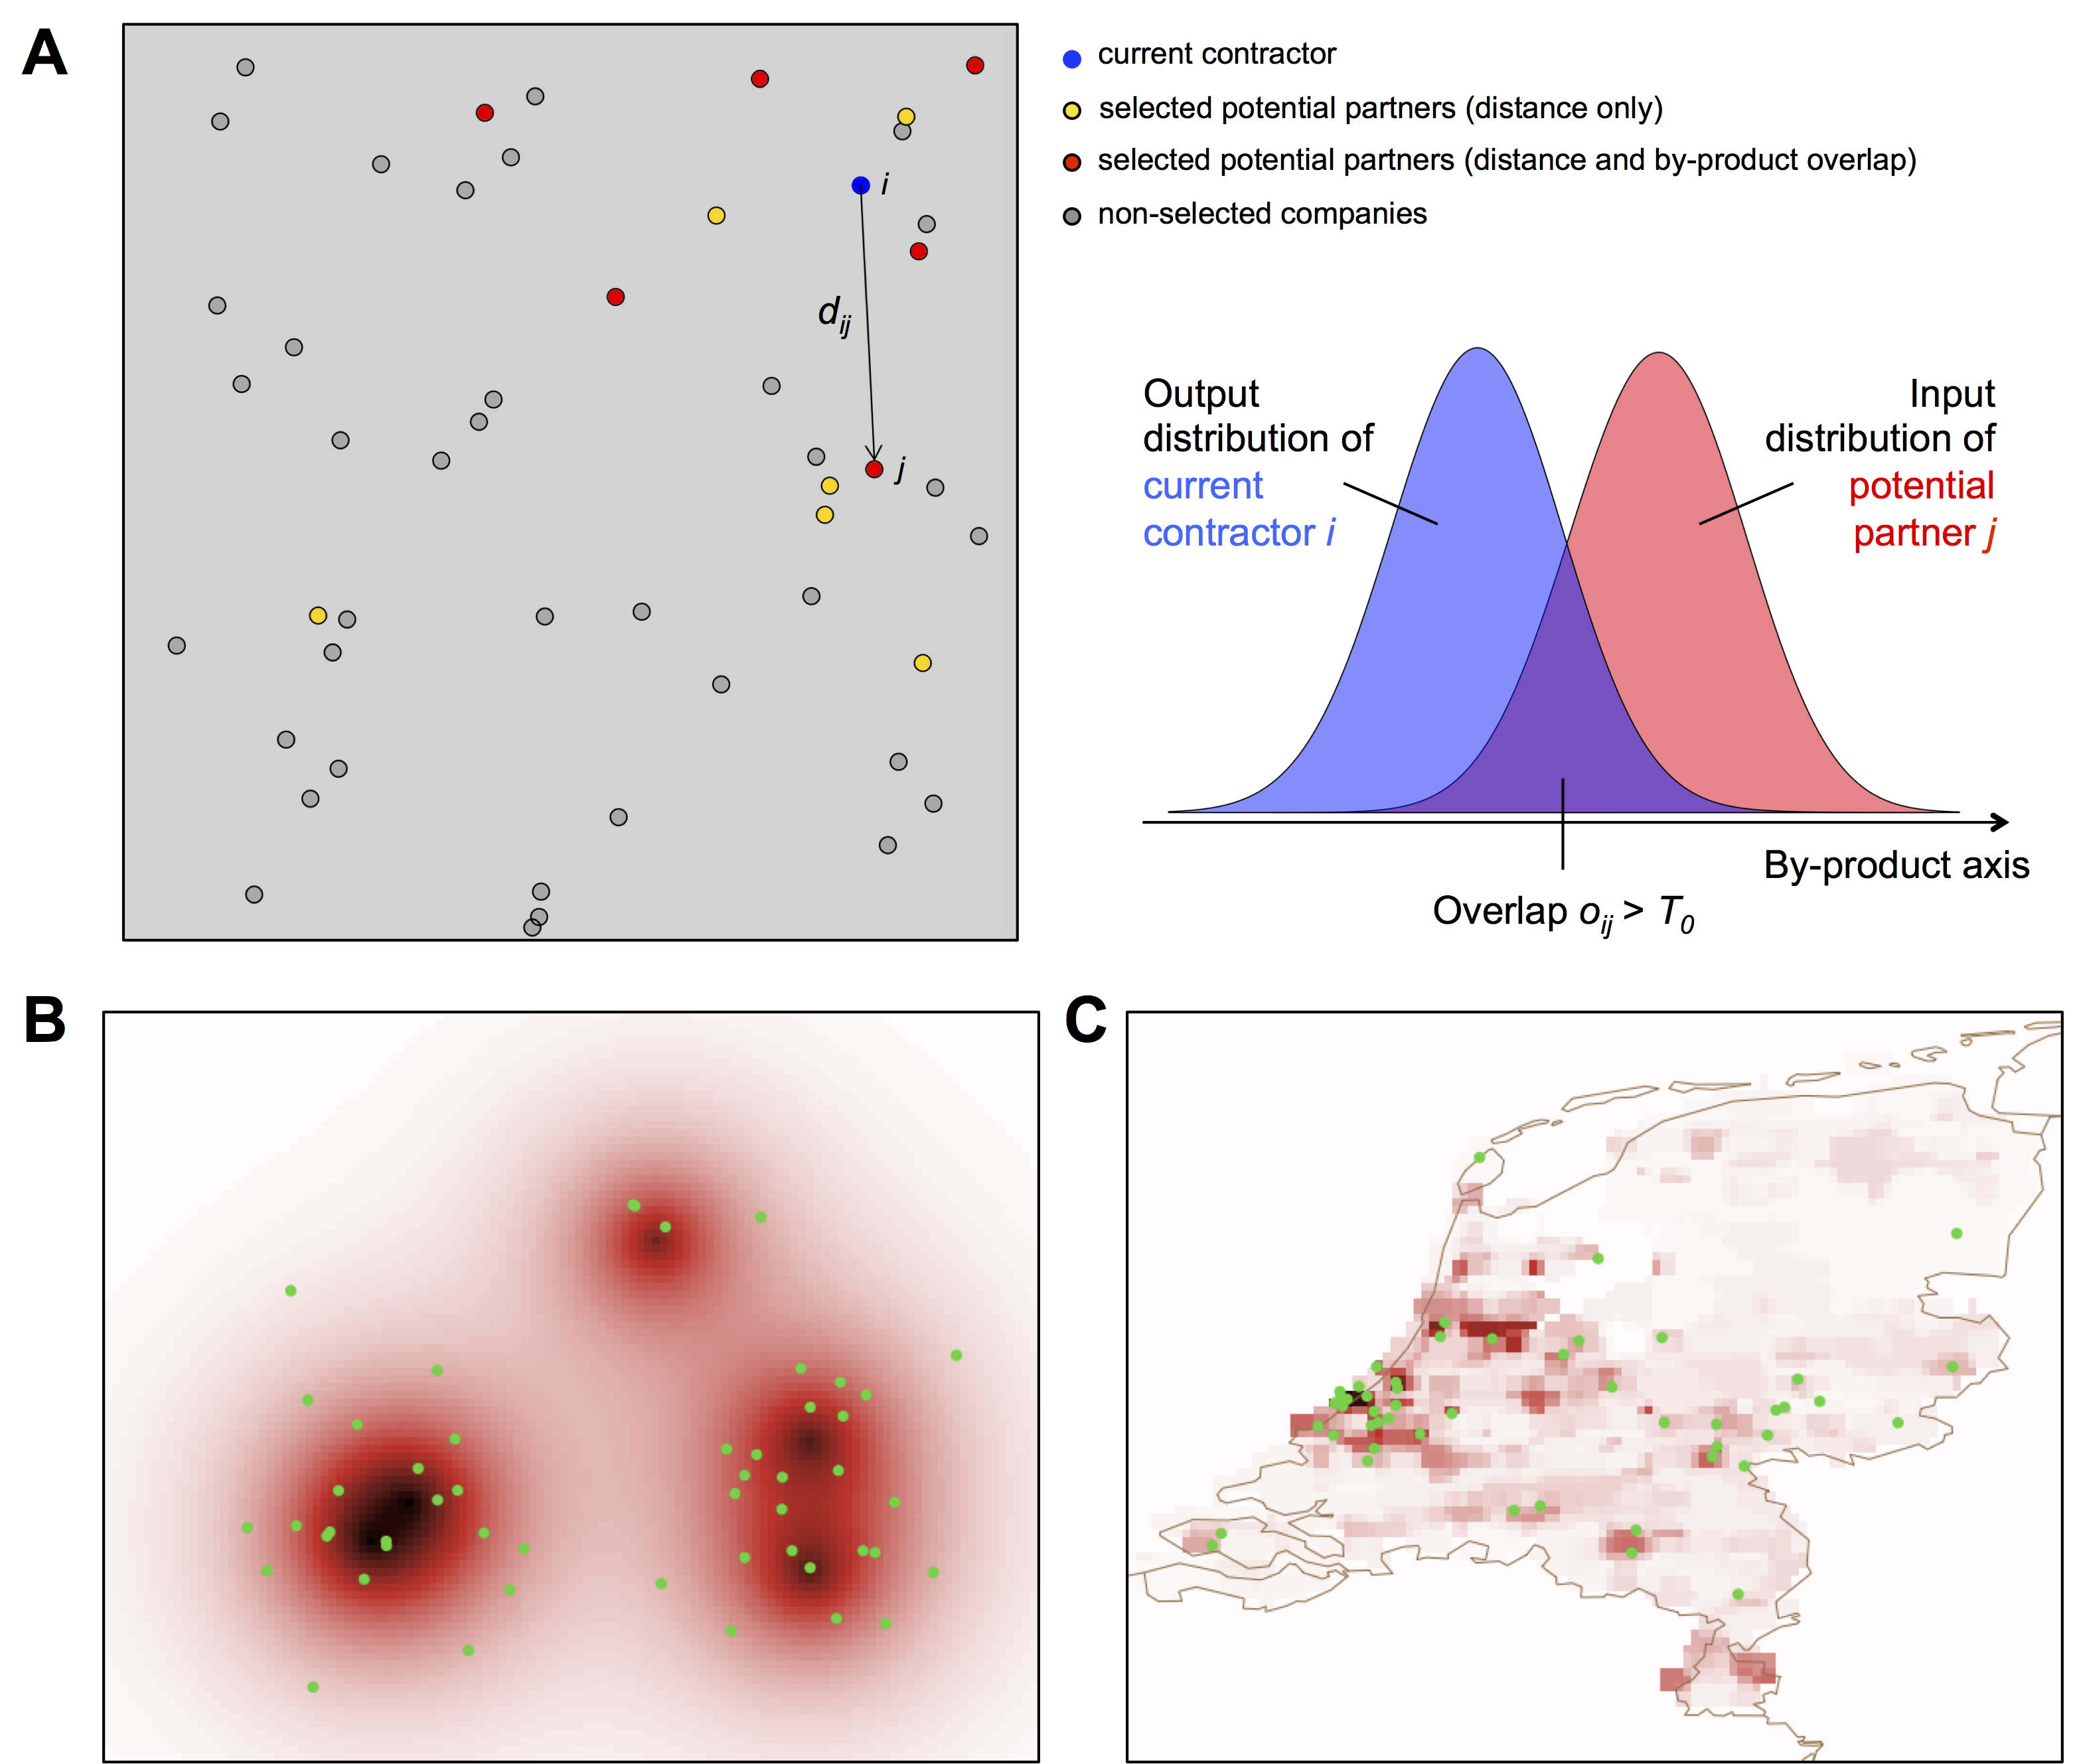
\includegraphics[width=0.55\textwidth]{figures/circulareconomy.png}
\end{center}


\textit{Agent-based modeling for circular economy processes from an interdisciplinary viewpoint}

\bigskip

\tiny

Raimbault, J., Broere, J., Somveille, M., Serna, J. M., Strombom, E., Moore, C., Zhu, B. \& Sugar, L. (2020). A spatial agent based model for simulating and optimizing networked eco-industrial systems. Resources, Conservation and Recycling, 155, 104538.

\nocite{raimbault2020spatial}

}


\sframe{Transportation governance}{

\begin{center}
	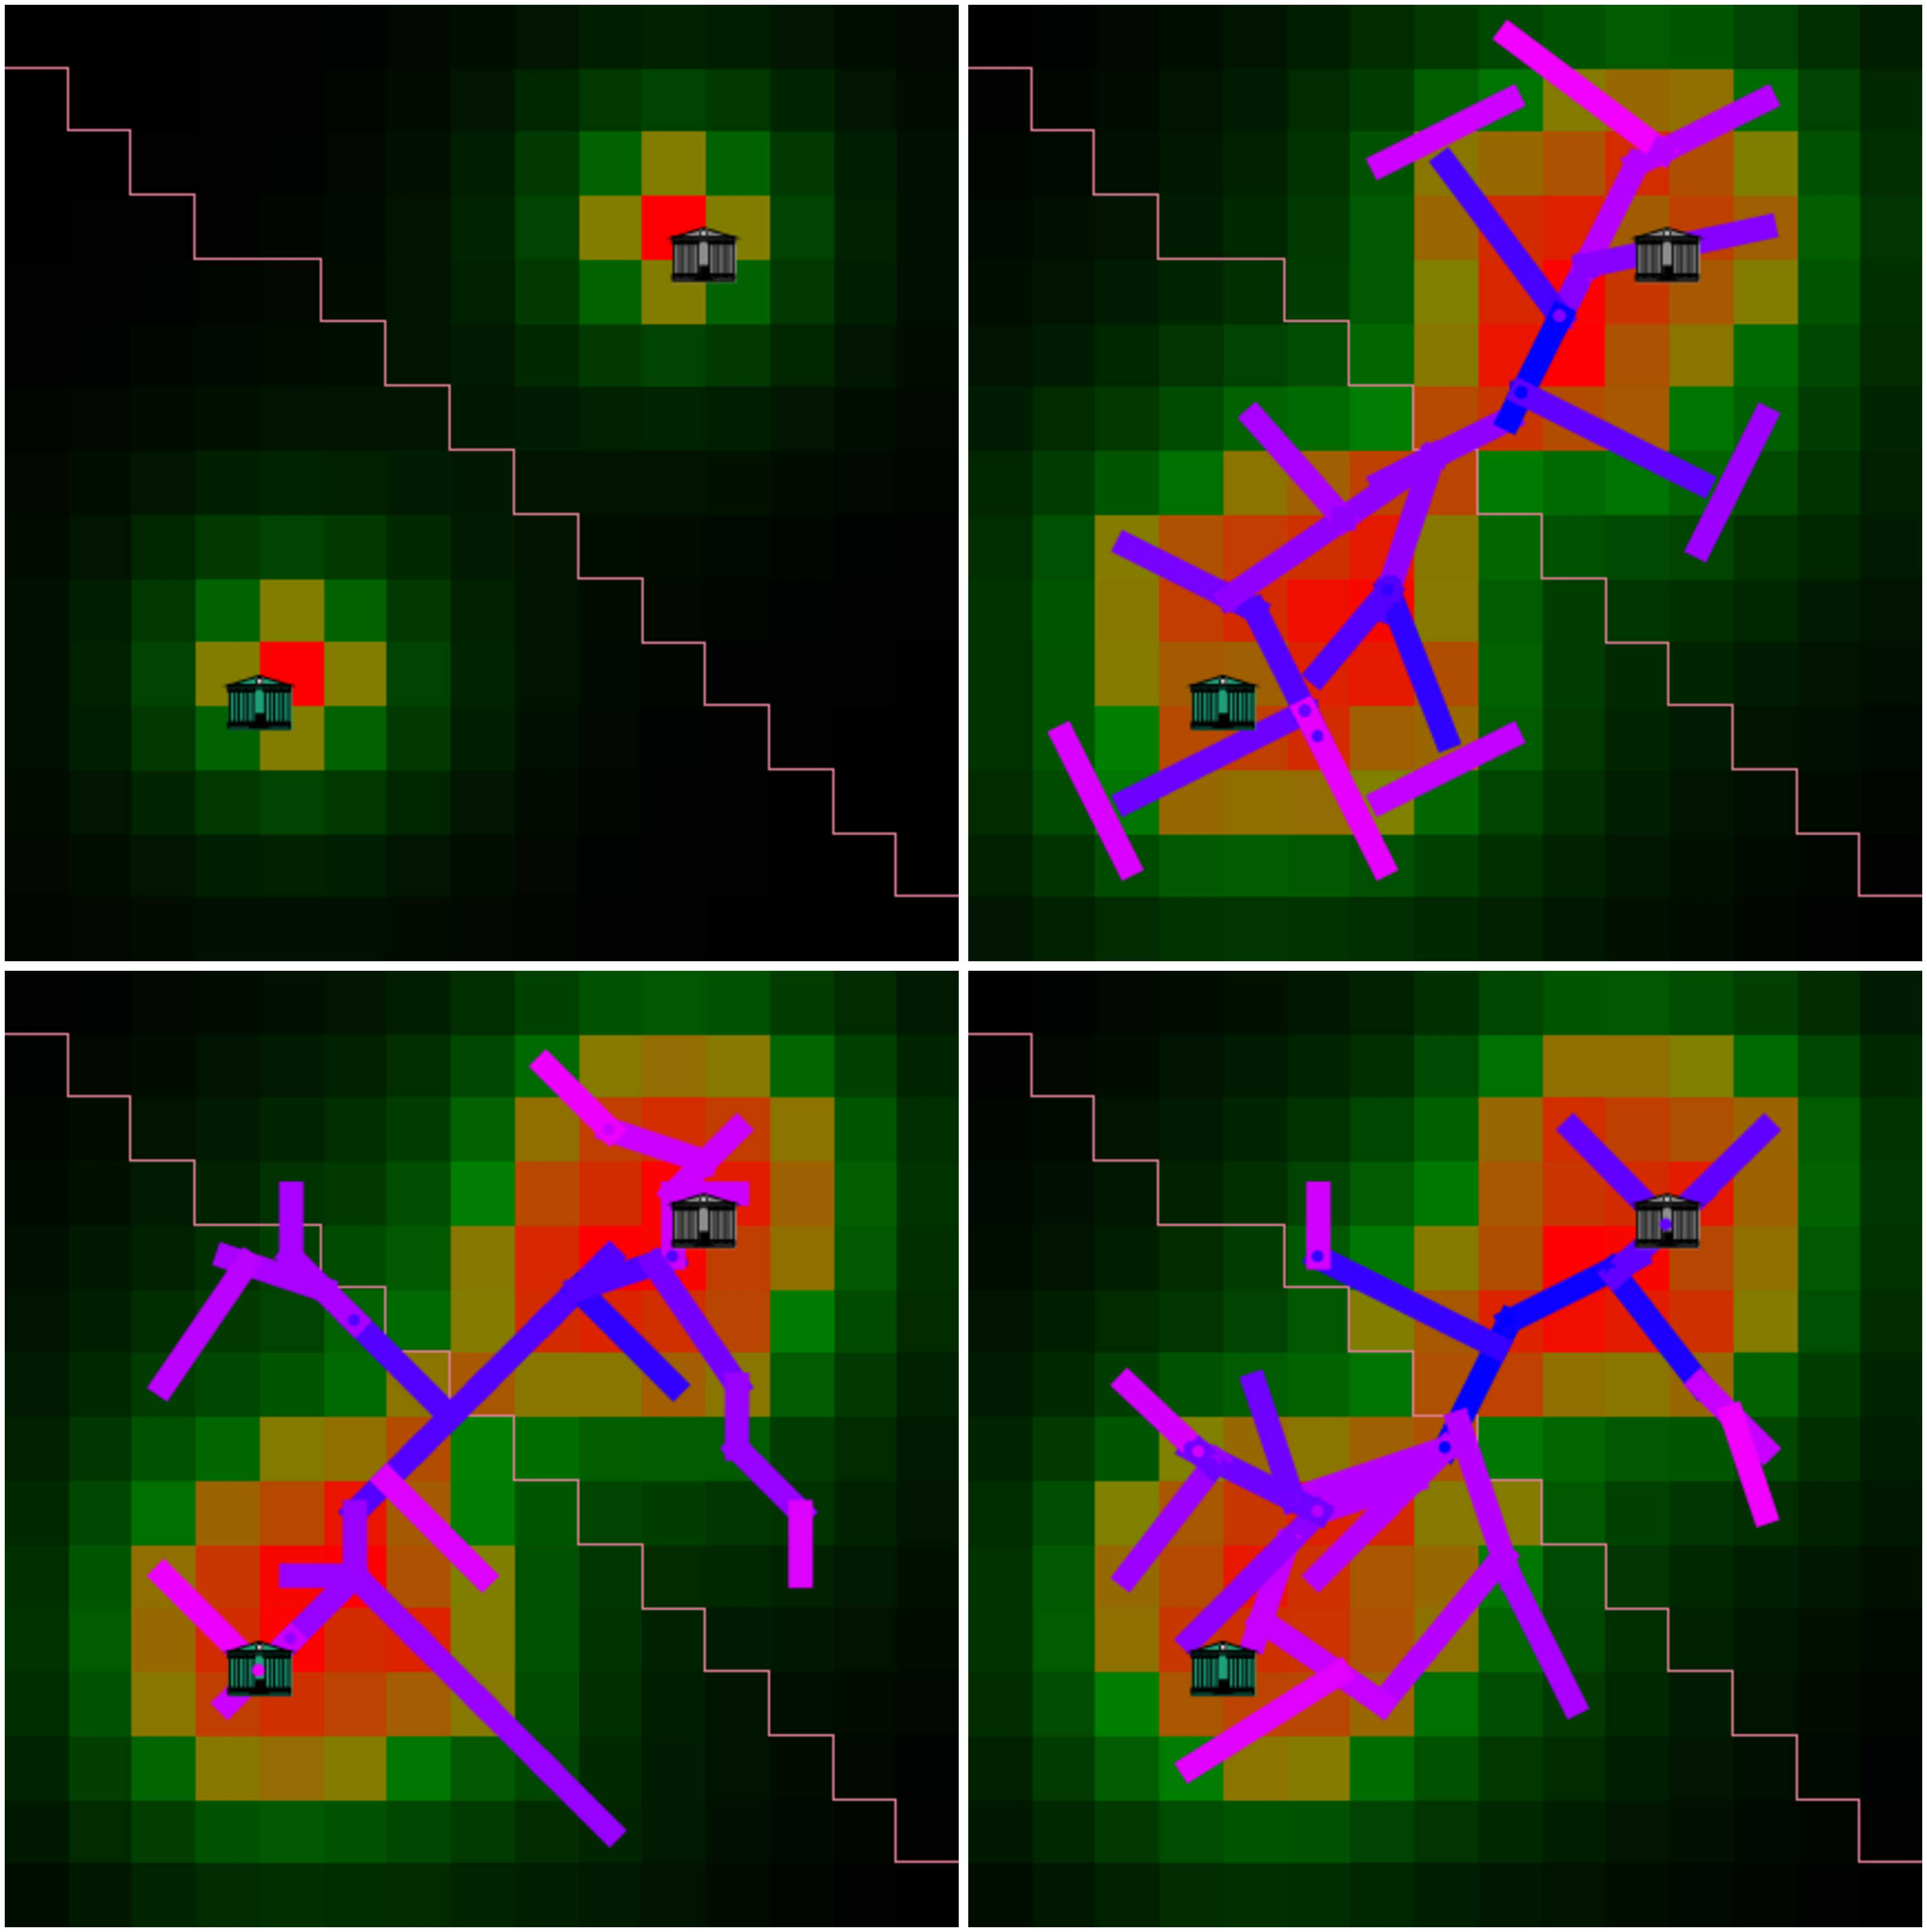
\includegraphics[width=0.5\textwidth]{figures/7-3-3-fig-lutecia-governance.jpg}
\end{center}

\textit{Simulating the decision-making processes of transport governance stakeholders}

\bigskip

\tiny

Raimbault, J., \& Le Néchet, F. (2021). Introducing endogenous transport provision in a LUTI model to explore polycentric governance systems. Journal of Transport Geography, 94, 103115.

\nocite{raimbault2021introducing}

}




\sframe{Spatial sensitivity analysis}{



\centering

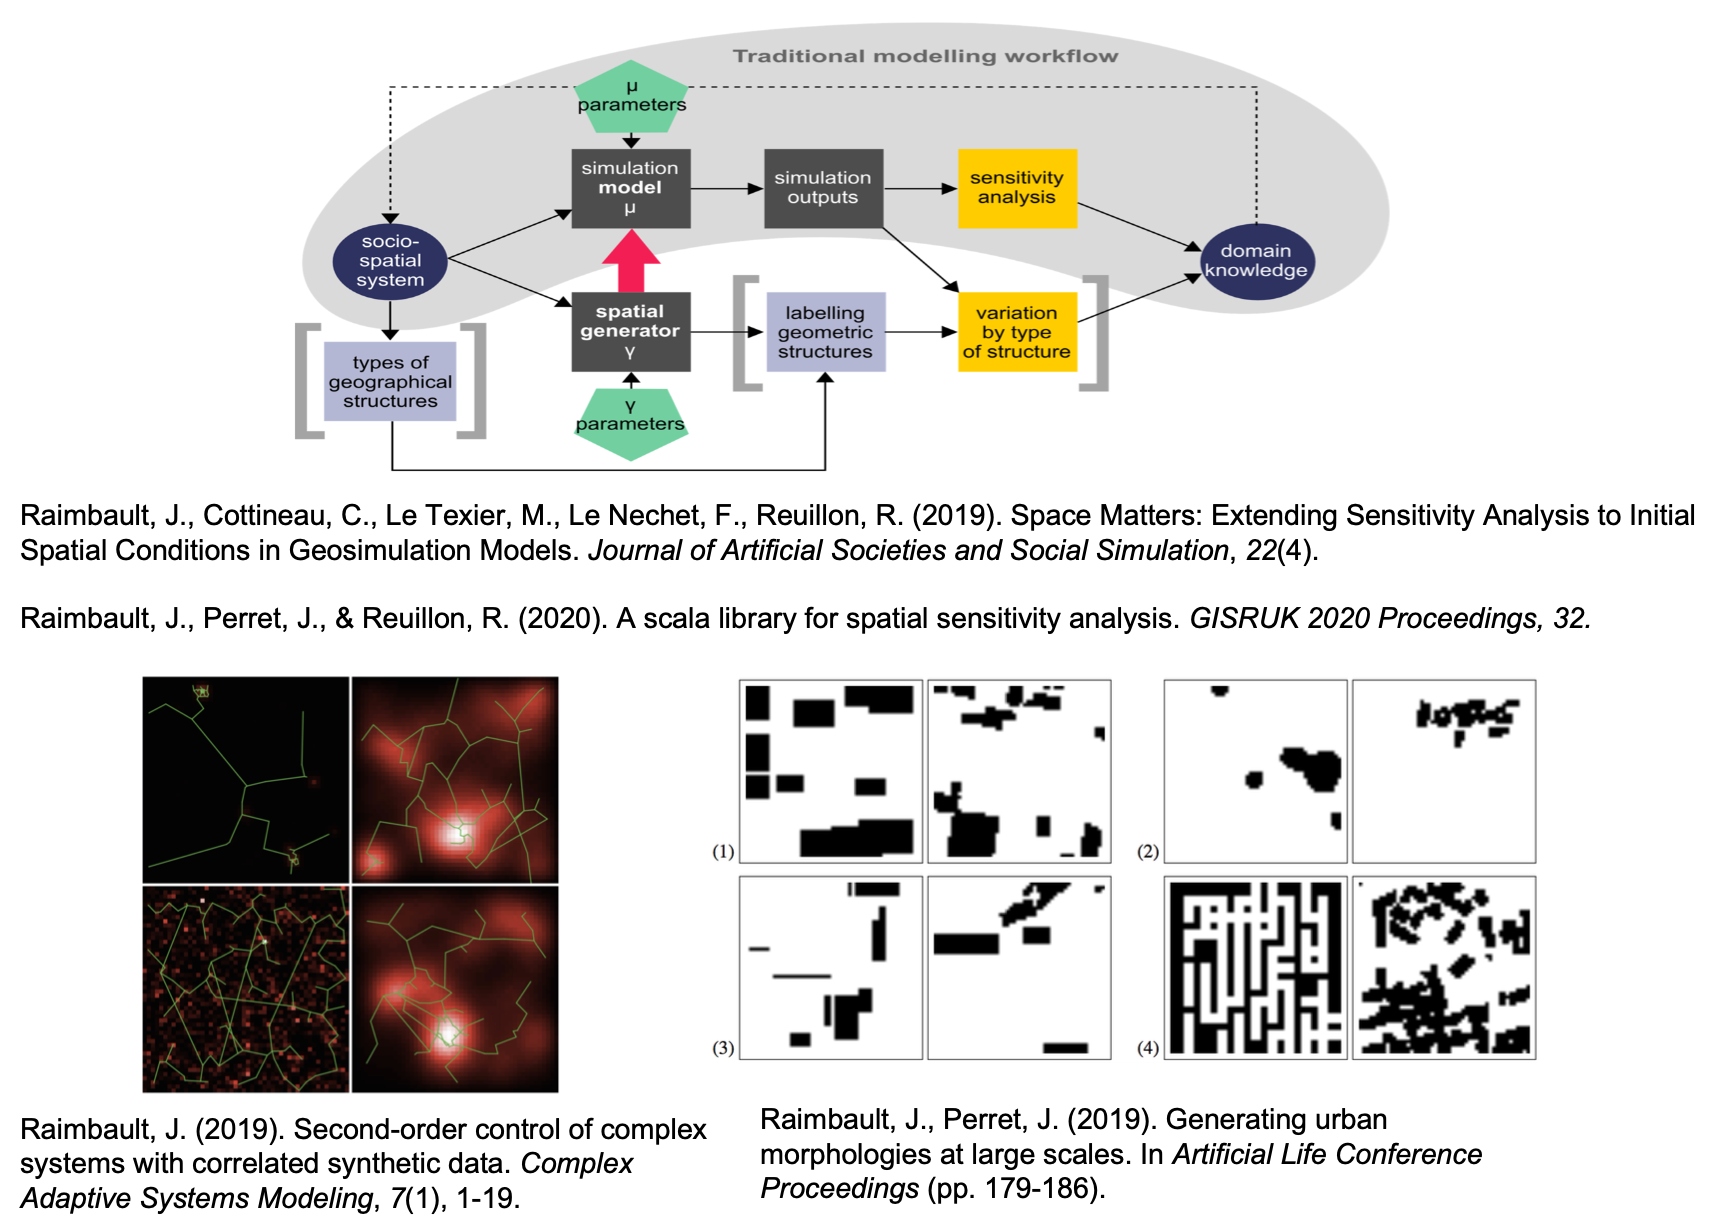
\includegraphics[width=0.95\linewidth]{figures/spatial_sa.png}

\nocite{raimbault2019second}
\nocite{raimbault2019generating}
\nocite{raimbault2019space}

}


\sframe{Quantitative epistemology}{

\justify

\vspace{-1cm}
\begin{center}
	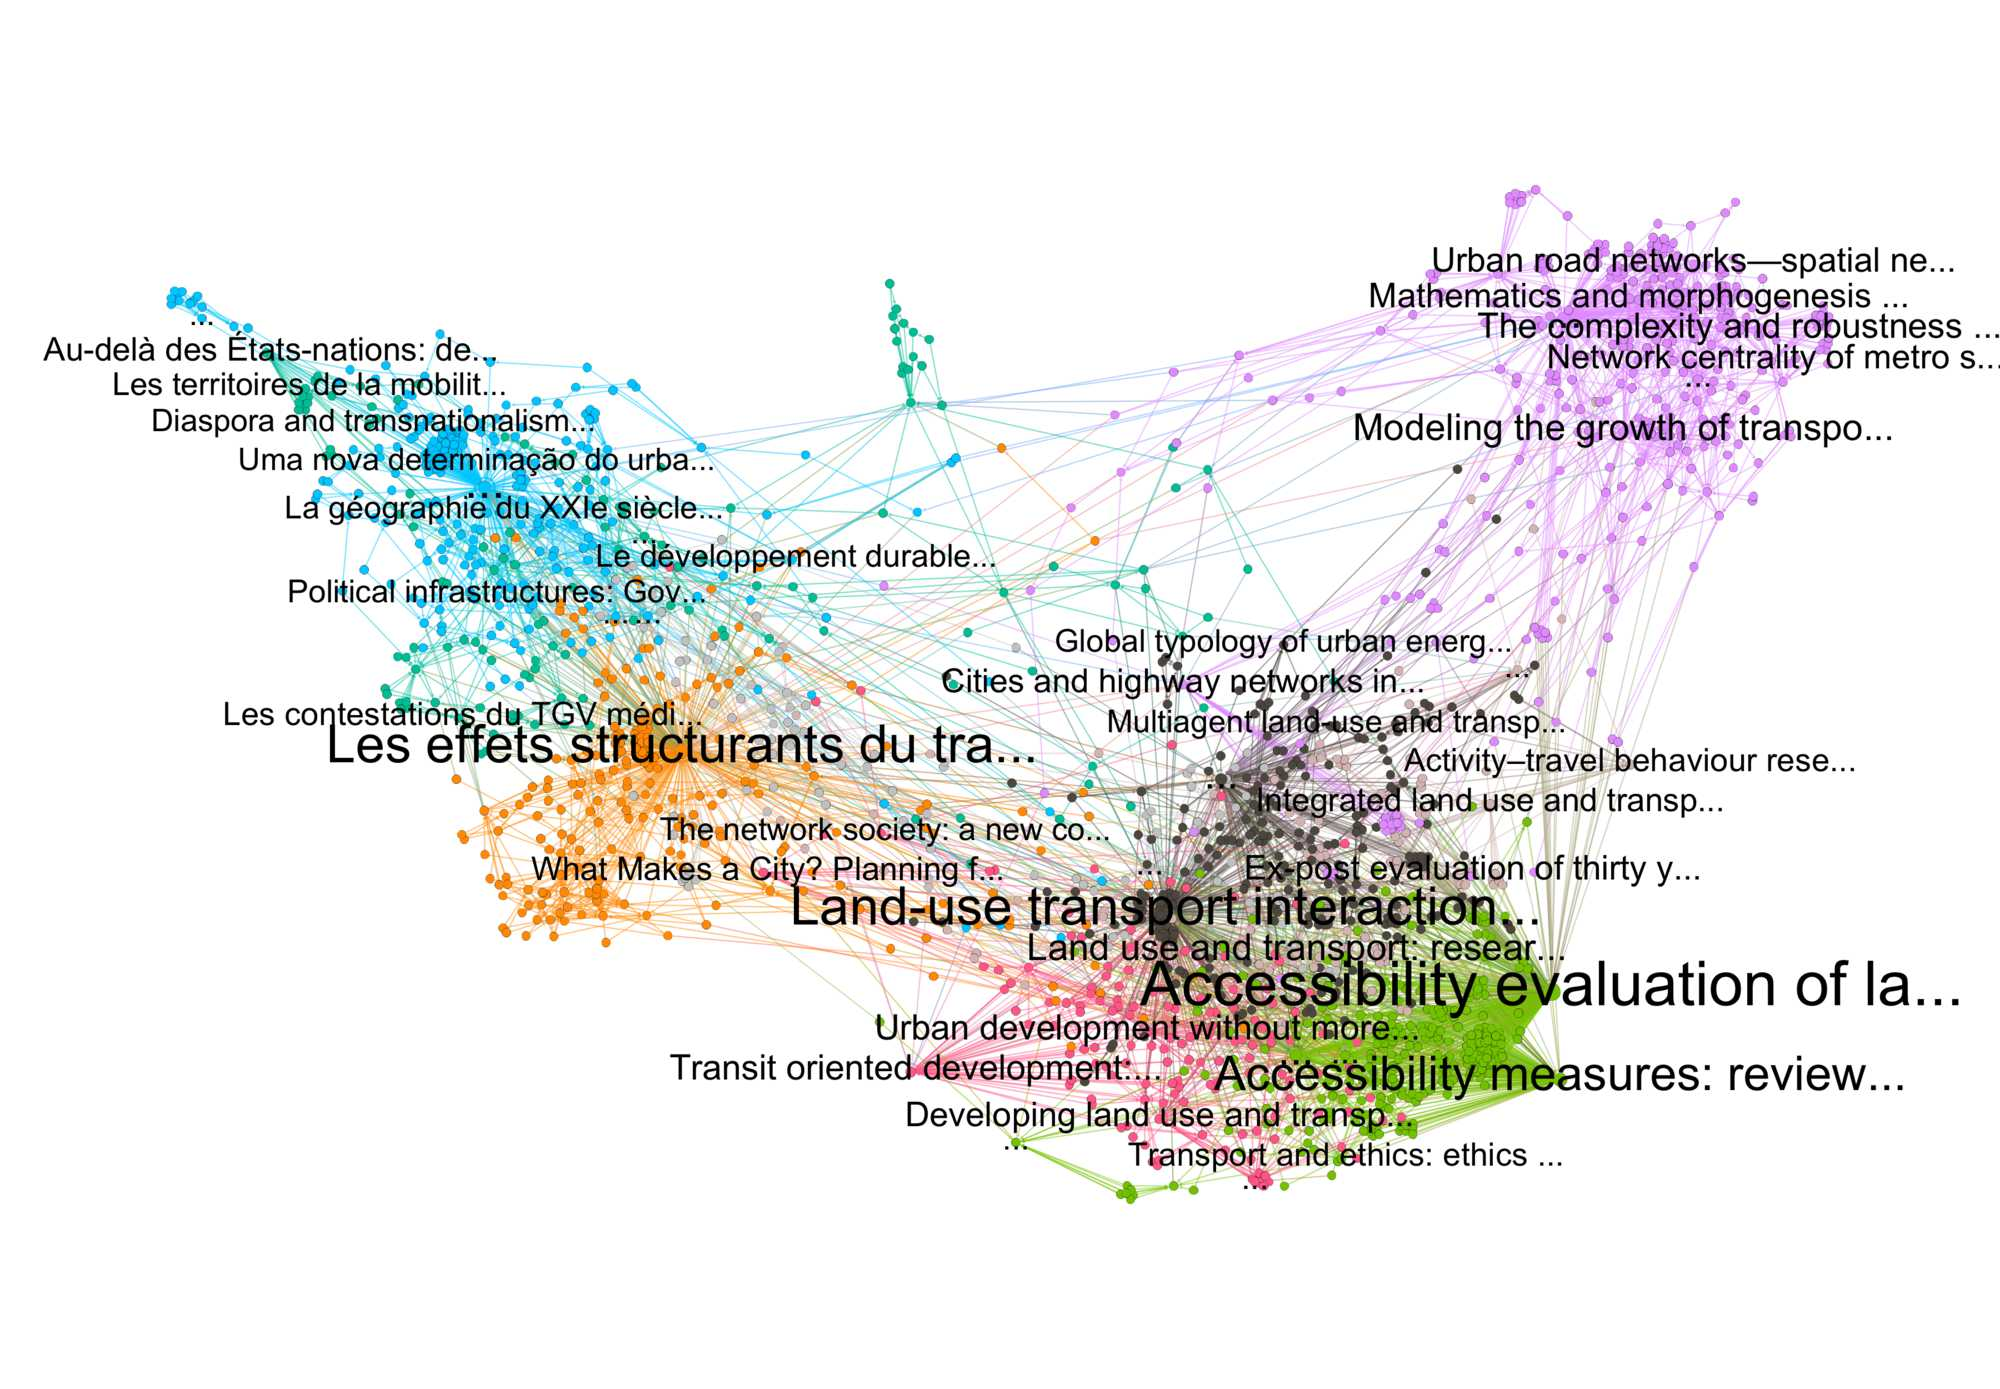
\includegraphics[width=0.9\textwidth,trim={0 2cm 0 2cm},clip]{figures/2-2-2-fig-quantepistemo-citnw.jpg}	
\end{center}

\smallskip

\vspace{-1cm}

\textit{Machine learning and natural language processing for knowledge mapping}

\medskip

\tiny

Raimbault, J. (2019). Exploration of an interdisciplinary scientific landscape. Scientometrics, 119(2), 617-641.

\smallskip

Bergeaud, A., Potiron, Y., \& Raimbault, J. (2017). Classifying patents based on their semantic content. PloS one, 12(4), e0176310.

\smallskip

Raimbault, J., Chasset, P. O., Cottineau, C., Commenges, H., Pumain, D., Kosmopoulos, C., \& Banos, A. (2021). Empowering open science with reflexive and spatialised indicators. Environment and Planning B: Urban Analytics and City Science, 48(2), 298-313.

}






\section{Project}


%\sframe{Systèmes urbains durables}{
%
%\justify

%\textbf{Définition}

%\bigskip

%$\rightarrow$ Approche classique de la durabilité: objectifs multiples (environnemental, sociologique, économique) souvent contradictoires
 
%\medskip 
 
%$\rightarrow$ Mis en oeuvre par des acteurs à différentes échelles, dans un contexte d'asymétrie d'information et de pouvoir

%\medskip

%$\rightarrow$ Adaptatifs sur de multiples échelles temporelles

%\bigskip

%\textbf{Pourquoi des modèles ?}

%\begin{center}
%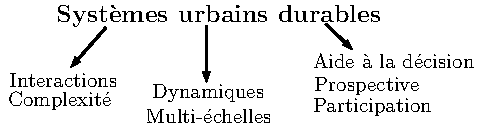
\includegraphics[width=\textwidth]{figures/def.pdf}
%\end{center}


%}



\sframe{Research project}{

\justify

\textbf{Sustainable urban systems: } (i) multiple contradictory objectives; (ii) implemented by stakeholders at different scales, within various information and power contexts; (iii) adaptive on multiple time scales.


\bigskip

\textbf{Models are essential tools to } (i) capture complexity; (ii) construct integrated perspectives; (iii) link data, empirical stylised facts and decision-making.

\bigskip


$\rightarrow$ \textbf{Integrated models} to simulate multiple dimensions of \textbf{urban systems} towards decision-making in the context of \textbf{sustainable transitions}.


}




\section{Axis}

\sframe{Project structure}{


\begin{center}
	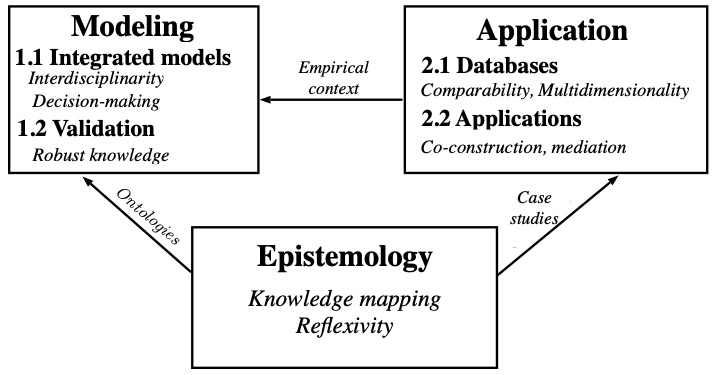
\includegraphics[width=\textwidth]{figures/axes_edited_EN.jpg}	
\end{center}



}


\sframe{Axis 1.1: Constructing integrated models}{



\textbf{Integrating models and theories}

\medskip

$\rightarrow$ Horizontal: interdisciplinarity, complementary dimensions

$\rightarrow$ Vertical: multiple scales of territorial systems

$\rightarrow$ Knowledge domains: multiple and hybrid methods


\bigskip

\textbf{Several open issues}

\medskip

$\rightarrow$ (In)compatibility of approaches

$\rightarrow$ Model coupling

$\rightarrow$ Multi-scale models




}


\sframe{Axis 1.2: Modeling methods}{



\textit{Simulation and high-performance computing: contribution to the OpenMOLE software} \hspace{0.5cm} 
\includegraphics[height=0.05\textheight]{figures/iconOM.png}
\includegraphics[height=0.05\textheight]{figures/openmole.png}


\bigskip

\textbf{Development of new methods:}

\medskip

$\rightarrow$ Methods for the validation of spatial simulation models

\medskip

$\rightarrow$ Optimisation and calibration methods (stochasticity)

\medskip

$\rightarrow$ Coupling simulation models with machine learning (surrogate models, hybrid methods)



\bigskip
\bigskip

\tiny

Raimbault, J., \& Pumain, D. (2019). Methods for Exploring Simulation Models. Geographical Modeling: Cities and Territories, 2, 125-150.


}



\sframe{Axis 2.1: Harmonised databases}{

\justify

\textit{Upstream integrated models}

\medskip

$\rightarrow$ Systematic review of existing databases for different SDGs

$\rightarrow$ Construction of open, harmonised and multidimensional databases, on consistent and comparable geographical entities

%\bigskip

\begin{table}[h]
	%\caption{Examples of databases related to different Sustainable Development Goals.}
	\begin{tabular}{|c|c|p{5.5cm}|}
	\hline
	Dimension & SDGs & Existing \\\hline
	Population & All & \textit{Global Human Settlement Layer} \cite{florczyk2019ghsl} \\
	GDP & 8 (Growth) & \cite{kummu2018gridded} \\
	Income & 10 (Inequalities) & \cite{van2014changing} \\
	Transport & 11 (Sustainable cities) & No harmonised dataset \\
	Emissions & 14 (Climate) & EDGAR \cite{janssens2019edgar} \\
	Innovation & 9 (Innovation) & No geolocated patent database\\\hline
	\end{tabular}
\end{table}

%\medskip

\footnotesize

\textit{Examples of different SDGs dimensions and existing databases}t


}

\sframe{Axis 2.2: Model applications}{

\justify

\textit{Downstream integrated models}

\bigskip

$\rightarrow$ Companion modeling, implication of stakeholders

\medskip

$\rightarrow$ Decision-making: interactive models for planning, exploration interfaces

\medskip

$\rightarrow$ Specific exploration methods (e.g. inverse problem)

\medskip

$\rightarrow$ Scientific mediation


}


\sframe{Axis 3: Knowledge mapping}{

\textit{Methods, tools and studies for open science and reflexivity}


\begin{center}
	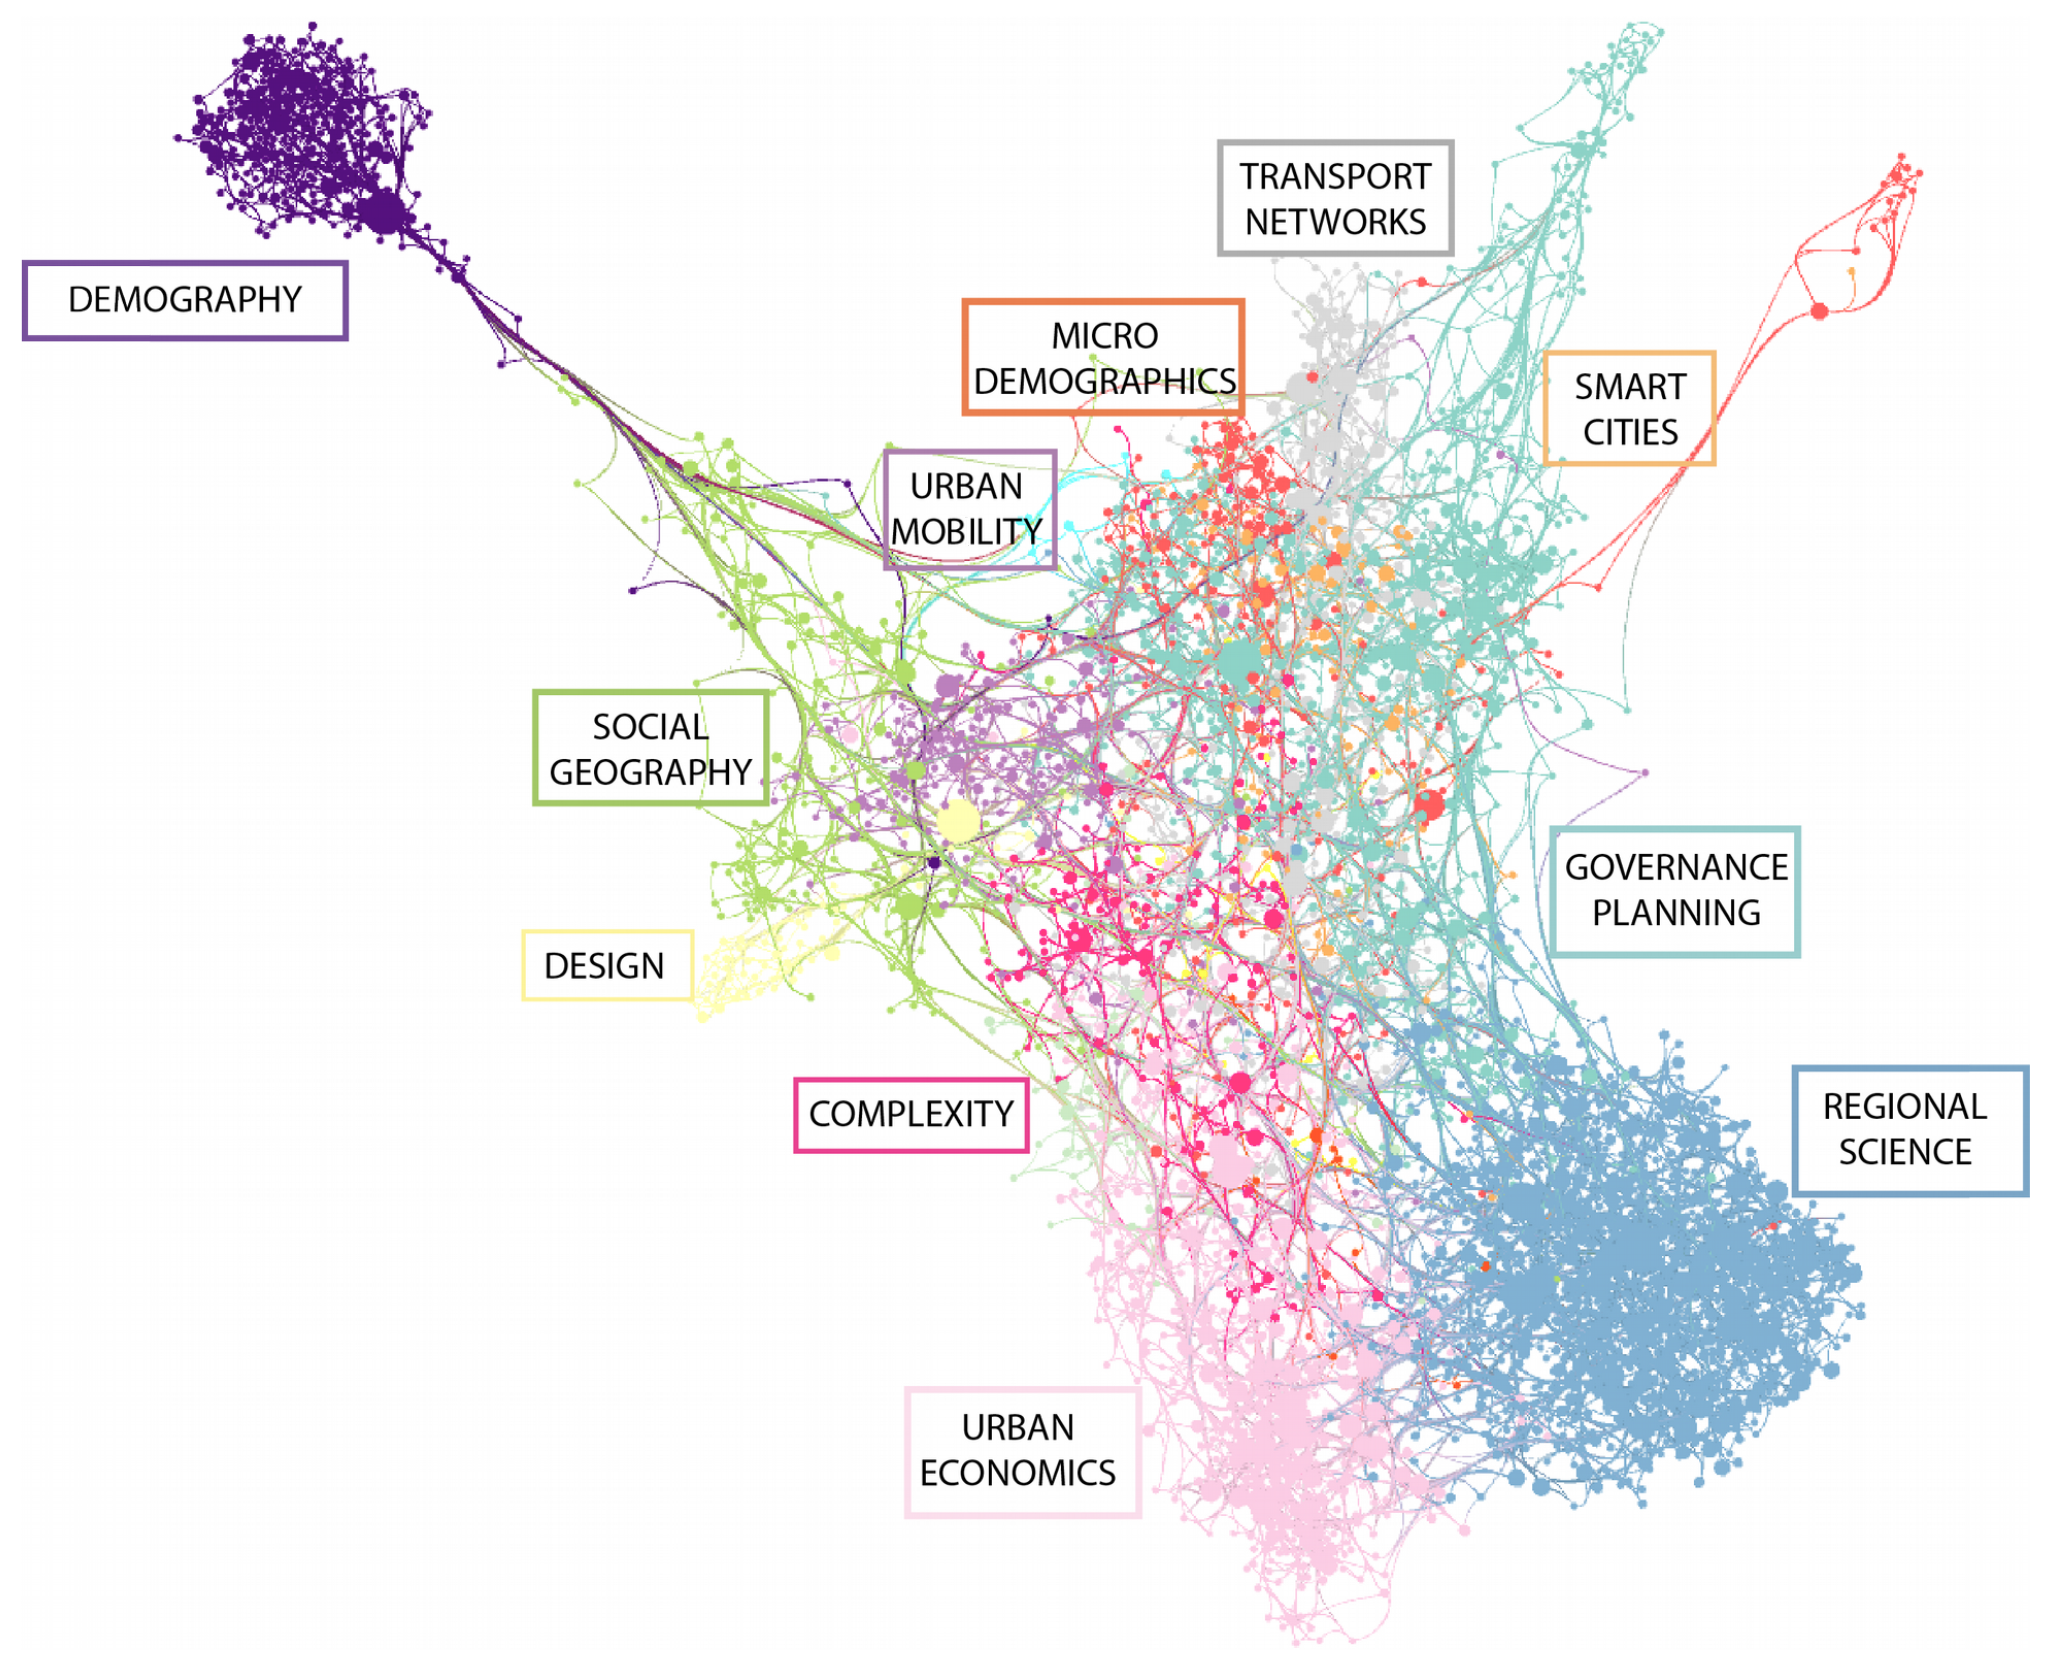
\includegraphics[height=0.7\textheight]{figures/urban-perspectives.png}
\end{center}


\medskip

\tiny

Pumain, D., \& Raimbault, J. (2020). Conclusion: Perspectives on Urban Theories. In Theories and Models of Urbanization (pp. 303-330). Springer, Cham.

\nocite{pumain2020conclusion}


}


\sframe{Implementing horizontal model integration}{

\justify

\textbf{Current work :} \textit{constructing a multimodal four step transport models by linking open components and data with scientific workflow engines}

\bigskip

\textbf{Integrated models:}

\begin{itemize}
	\item MATSim model (MATSim Community) for transport \cite{w2016multi}
	\item SPENSER model (University of Leeds) for synthetic population \cite{spooner2021dynamic}
	\item QUANT model (CASA, University College London) for spatial interactions \cite{batty2021new}
	\item spatialdata library (OpenMOLE community) for data processing \cite{raimbault2020scala}
\end{itemize}

\smallskip

\tiny

Raimbault, J., \& Batty, M. (2021). Estimating public transport congestion in UK urban areas with open transport models. GISRUK 2021 Proceedings.

\nocite{raimbault2021estimating}

}


\sframe{Horizontal integration: multi-modeling and benchmarks}{


\begin{center}
	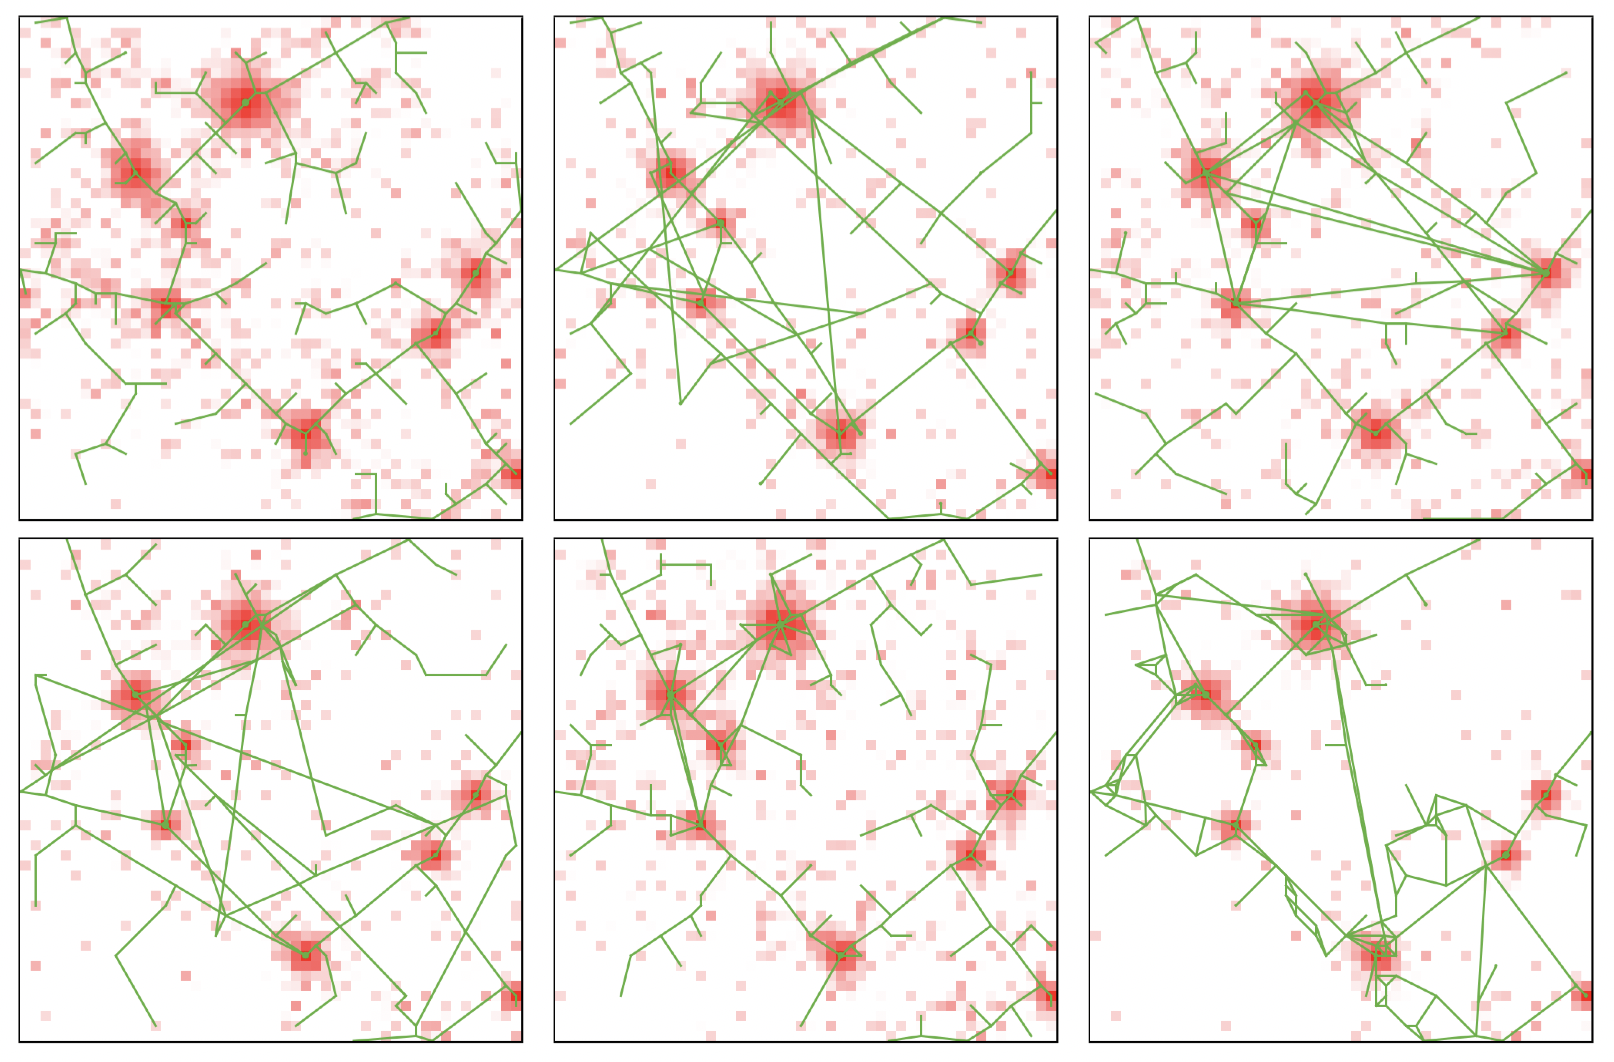
\includegraphics[width=0.56\linewidth]{figures/meso_multimodeling.png}\hspace{0.5cm}
	
\includegraphics[width=0.36\linewidth]{figures/mesobench_Fig3.png}
\end{center}

\medskip

\textit{Benchmarking network and urban morphogenesis models}


\medskip

\tiny

Raimbault, J. (2018). Multi-modeling the morphogenesis of transportation networks. In Artificial Life Conference Proceedings (pp. 382-383). MIT Press, Cambridge.

\nocite{raimbault2018multi}

\smallskip

Raimbault, J. (2020). A comparison of simple models for urban morphogenesis. arXiv preprint arXiv:2008.13277.

\nocite{raimbault2020comparison}

\smallskip

Raimbault, J. (2021). Complementarity of generative models for road networks. arXiv preprint arXiv:2109.15206.

\nocite{raimbault2021complementarity}



}



\sframe{Vertical integration: towards multi-scale models}{



\begin{center}
	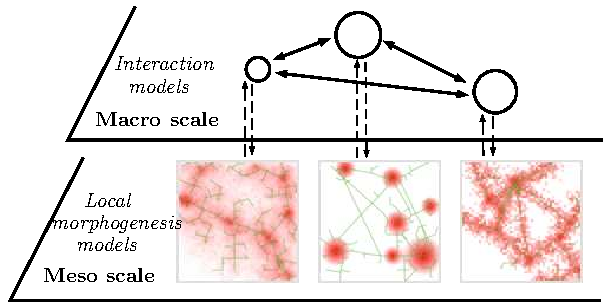
\includegraphics[width=0.75\textwidth]{figures/multiscale_morph.pdf}
\end{center}

\medskip

\textit{Processes specific to scales, coupling implies dedicated ontologies} 

\medskip

\tiny

Raimbault, J. (2021). Strong coupling between scales in a multi-scalar model of urban dynamics. arXiv preprint arXiv:2101.12725.

\nocite{raimbault2021strong}

\smallskip

Raimbault, J. (2021). A multiscale model of urban morphogenesis. arXiv preprint arXiv:2103.17241.

\nocite{raimbault2021multiscale}


}










\sframe{Towards knowledge integration: ERC Geodivercity}{

% presentation generale de Geodivercity

\begin{columns}
\begin{column}{0.4\textwidth}
	\centering
	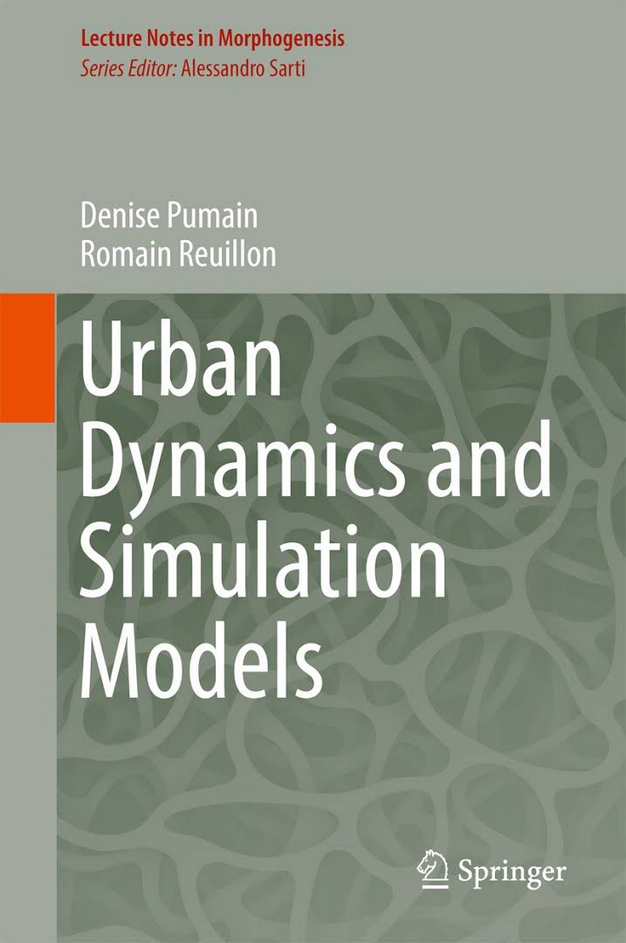
\includegraphics[width=0.9\textwidth]{figures/urban-dynamics-simulation-models-geodivercity.png}
\end{column}
\begin{column}{0.6\textwidth}
	Development of evolutive urban theory
	
	 \nocite{pumain2018evolutionary}
	
	\medskip

	$\rightarrow$ Recurrent stylized facts on main systems of cities
	
	$\rightarrow$ Construction of simulation models (with an explicative purpose)
	
	$\rightarrow$ Tools and methods to explore simulation models
	
	\smallskip
	
	
\includegraphics[width=\textwidth]{figures/openmole.png}
		
	
\end{column}
\end{columns}

\bigskip
\tiny

Pumain, D. (2018). An evolutionary theory of urban systems. In International and Transnational Perspectives on Urban Systems (pp. 3-18). Springer, Singapore.


}


\sframe{Iterative construction of knowledge across domains}{


\begin{center}
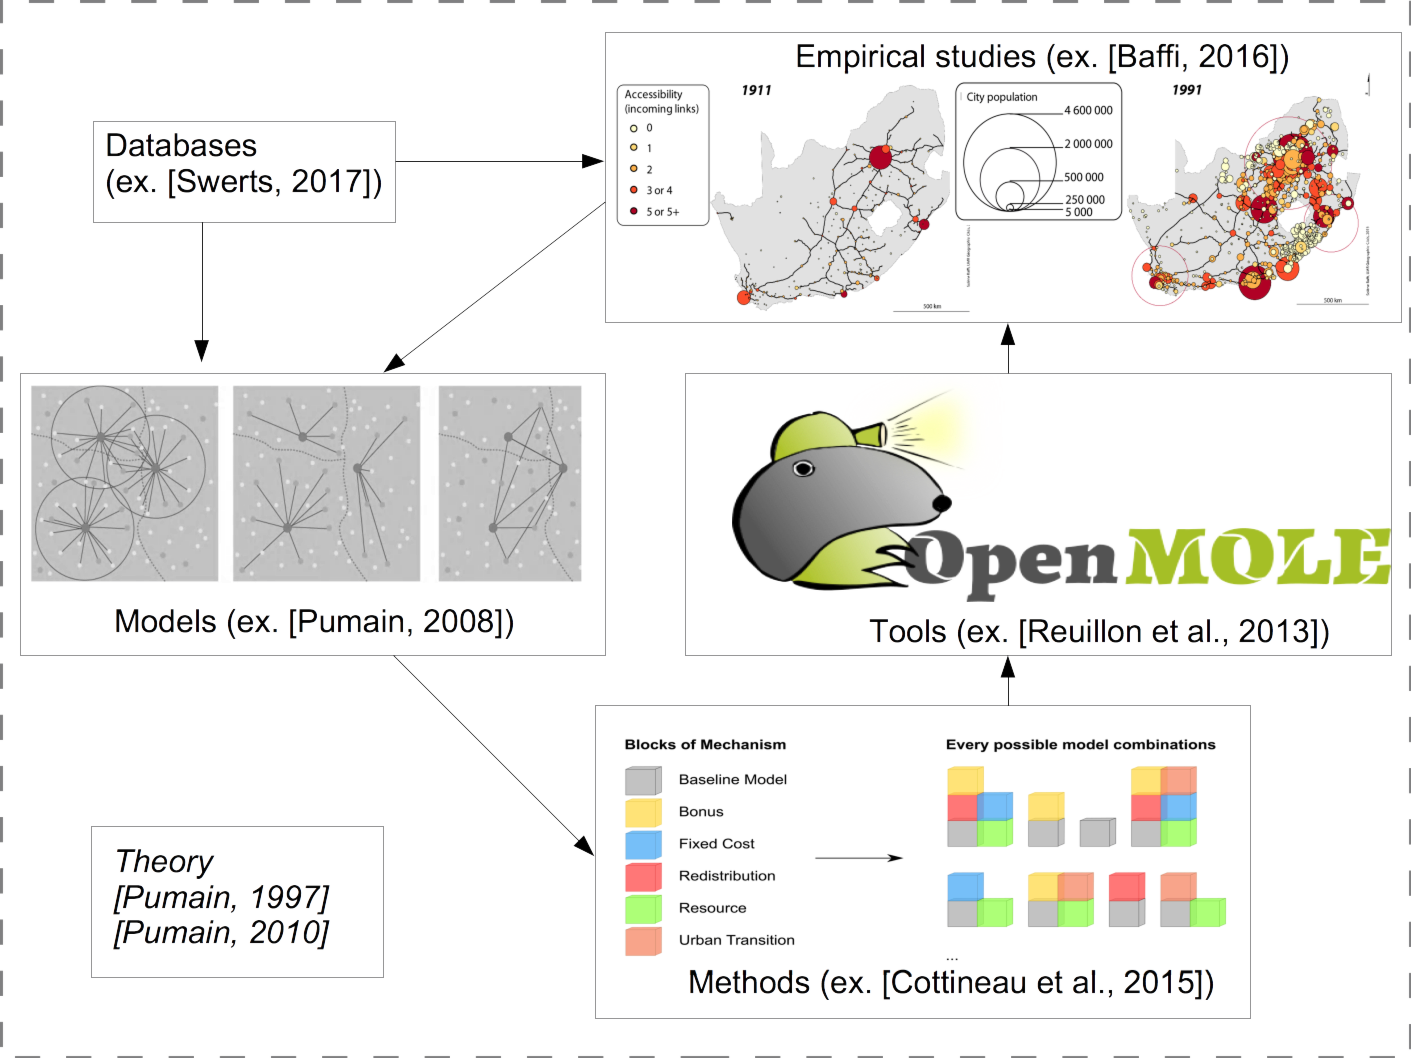
\includegraphics[height=0.75\textheight]{figures/openmoleslide}
\end{center}

\medskip

\tiny

Raimbault, J. (2017). An Applied Knowledge Framework to Study Complex Systems. In Complex Systems Design \& Management (pp. 31-45).

\nocite{raimbault2017applied}


\nocite{baffi:tel-01389347}
\nocite{pumain2008socio}
\nocite{reuillon2013openmole}
\nocite{cottineau2015modular}
\nocite{swerts2017database}
\nocite{pumain1997pour}
\nocite{pumain2010theorie}

}



\sframe{Model exploration methods to foster knowledge integration}{
	
	\textit{(i) Innovative exploration methods; (ii) Scaling of methods on high performance computing environments; (iii) No interference with the model.}
	
	\smallskip
	
	\centering
	
	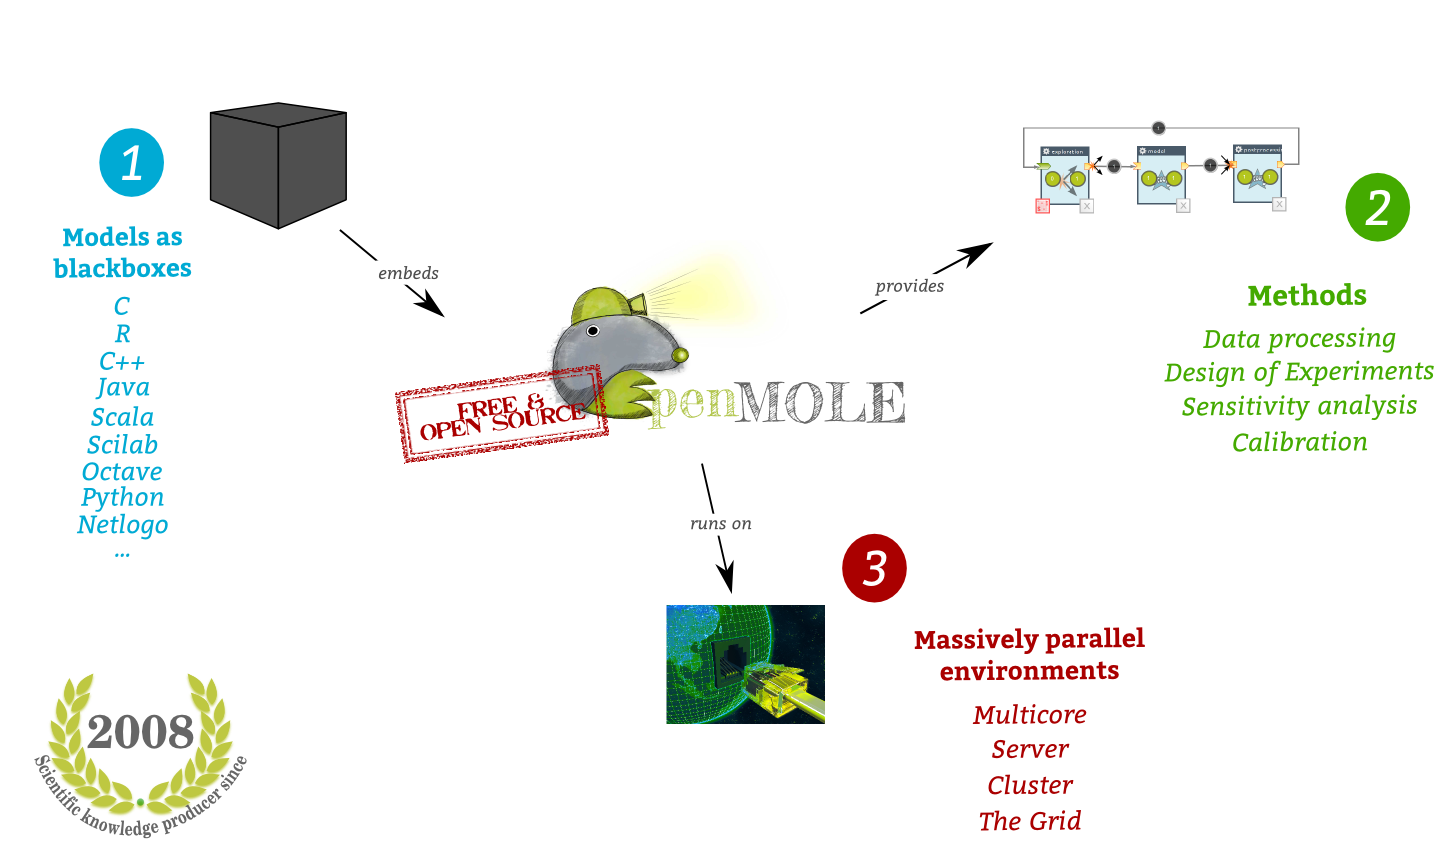
\includegraphics[width=\textwidth]{figures/openmoleGal.png}
	
}




\sframe{Towards models for sustainable policies}{

\textit{Benchmark of growth models for systems of cities} 

\nocite{raimbault2018systematic}

\centering

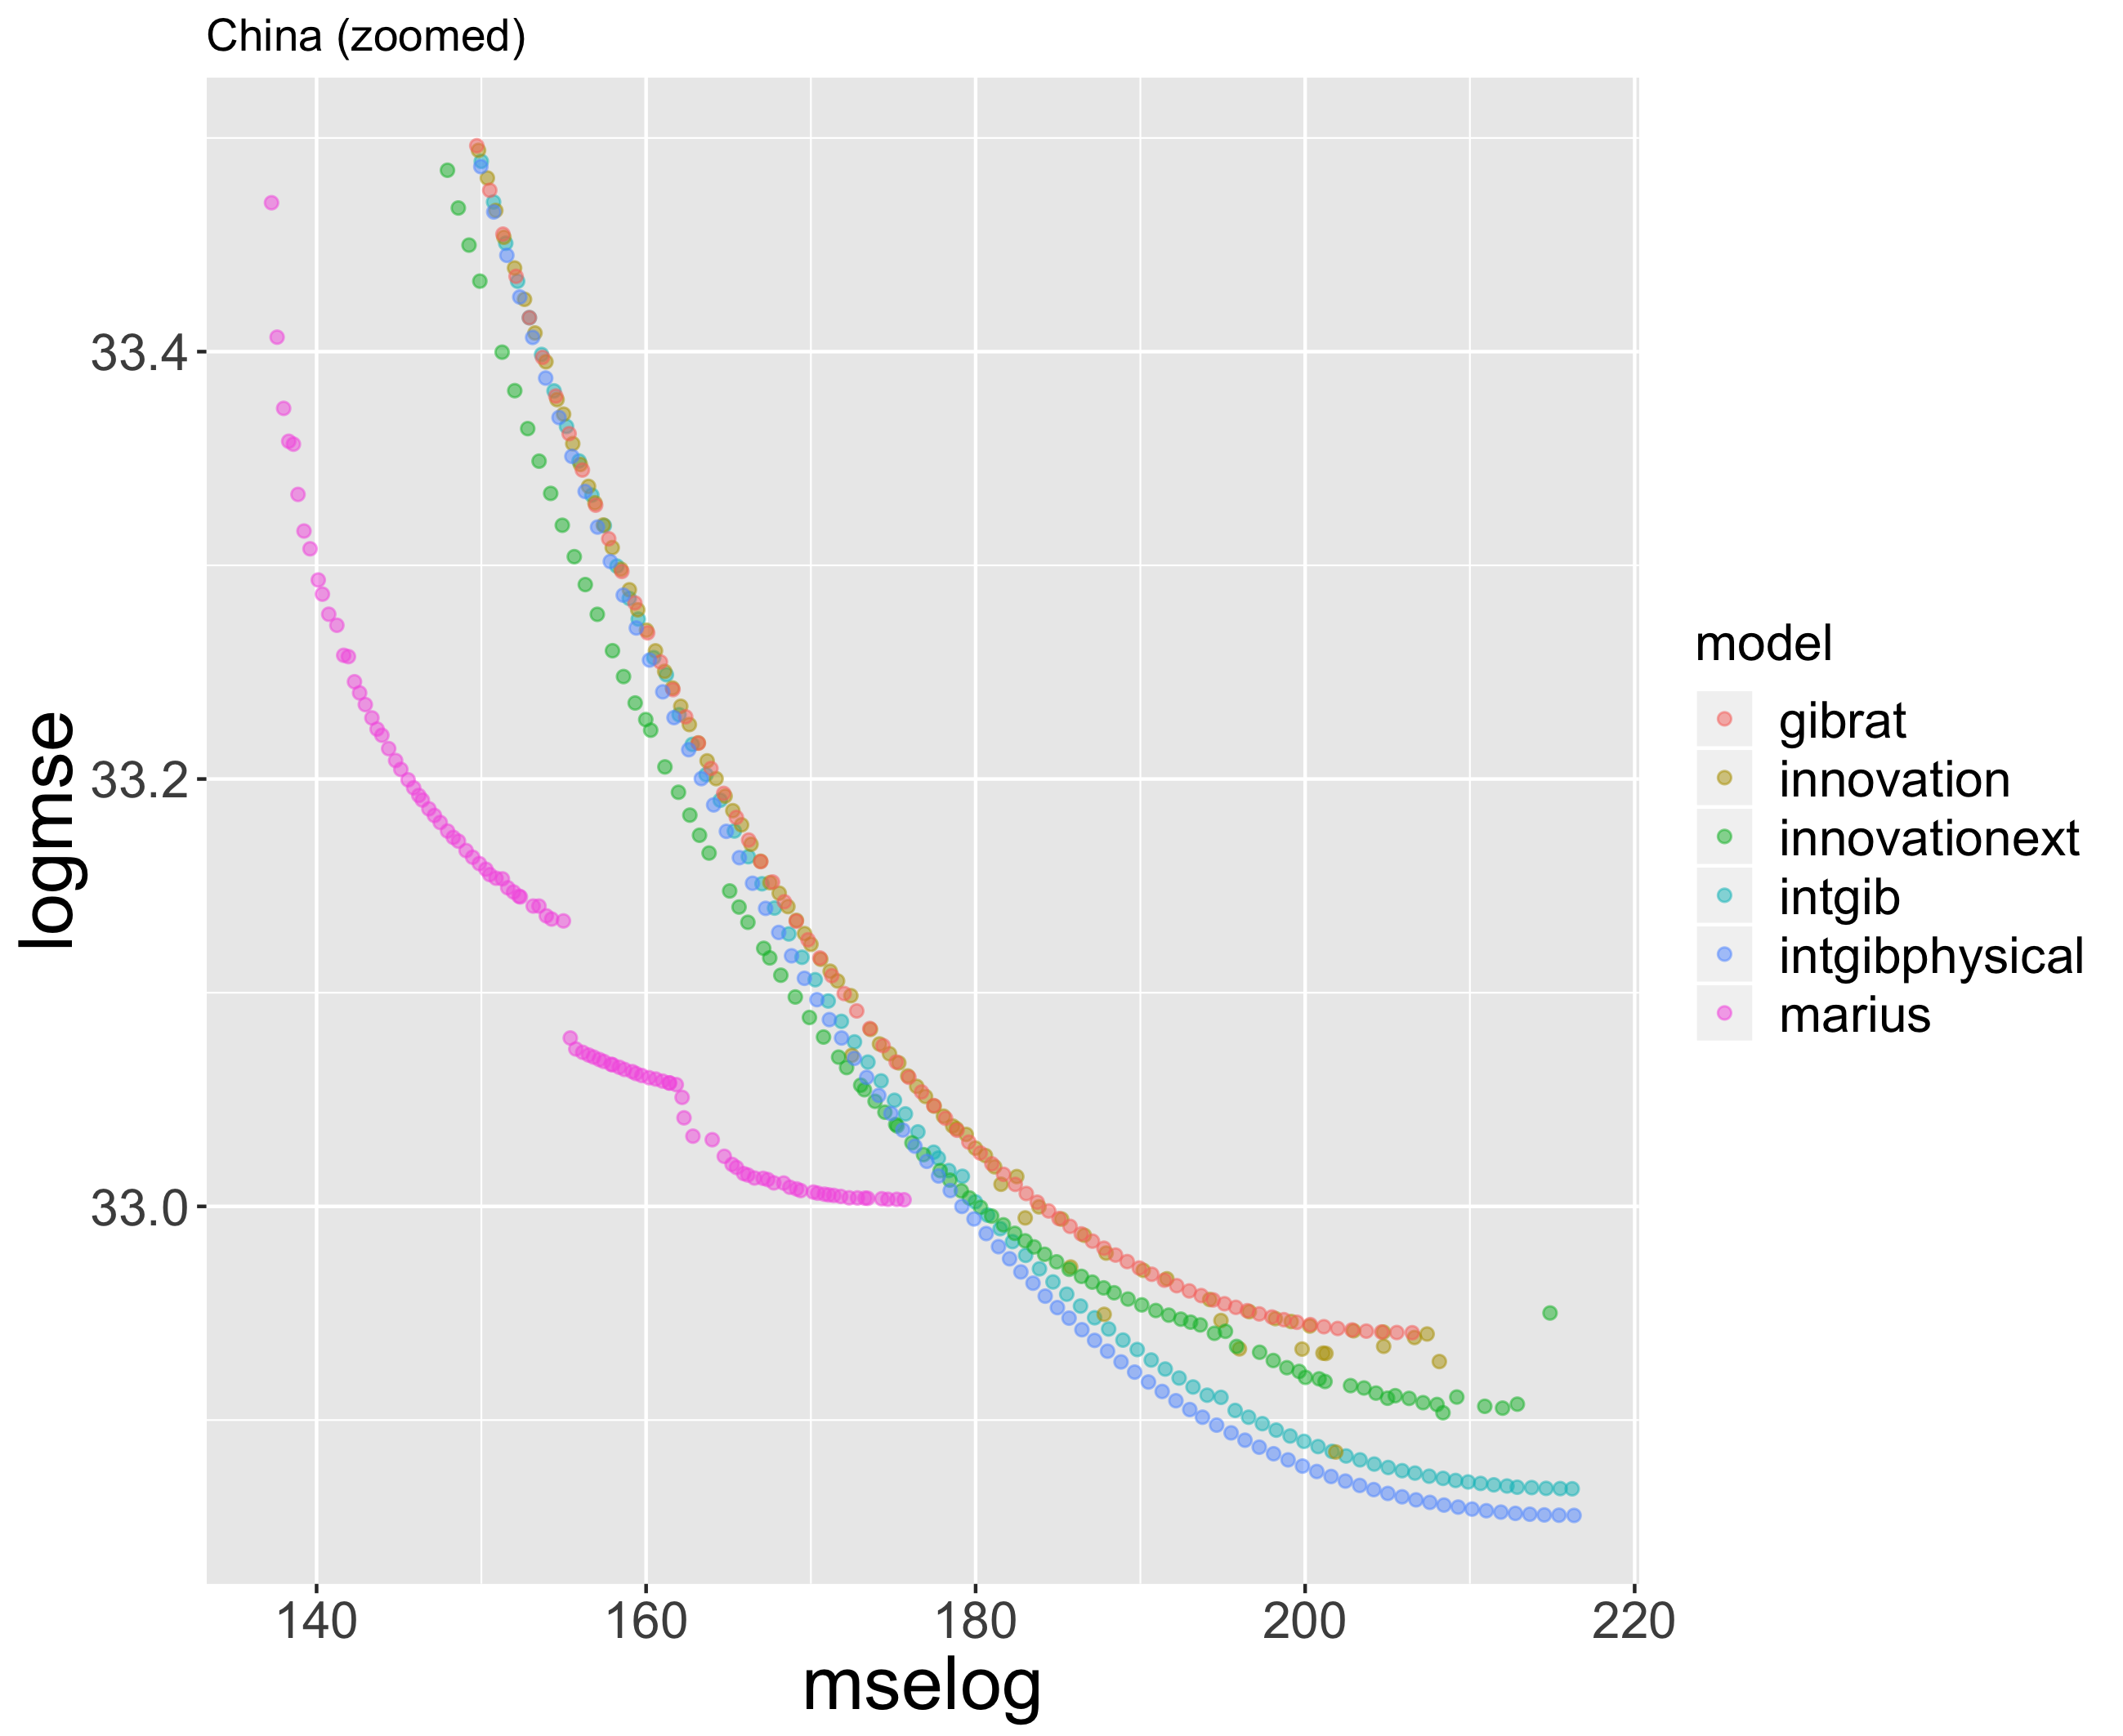
\includegraphics[width=0.85\textwidth]{figures/CN_zoomed.png}

}


\sframe{Towards models for sustainable policies}{

\textit{Identifying endogenous sustainable mega-city regions in Europe}

\medskip

% Marami
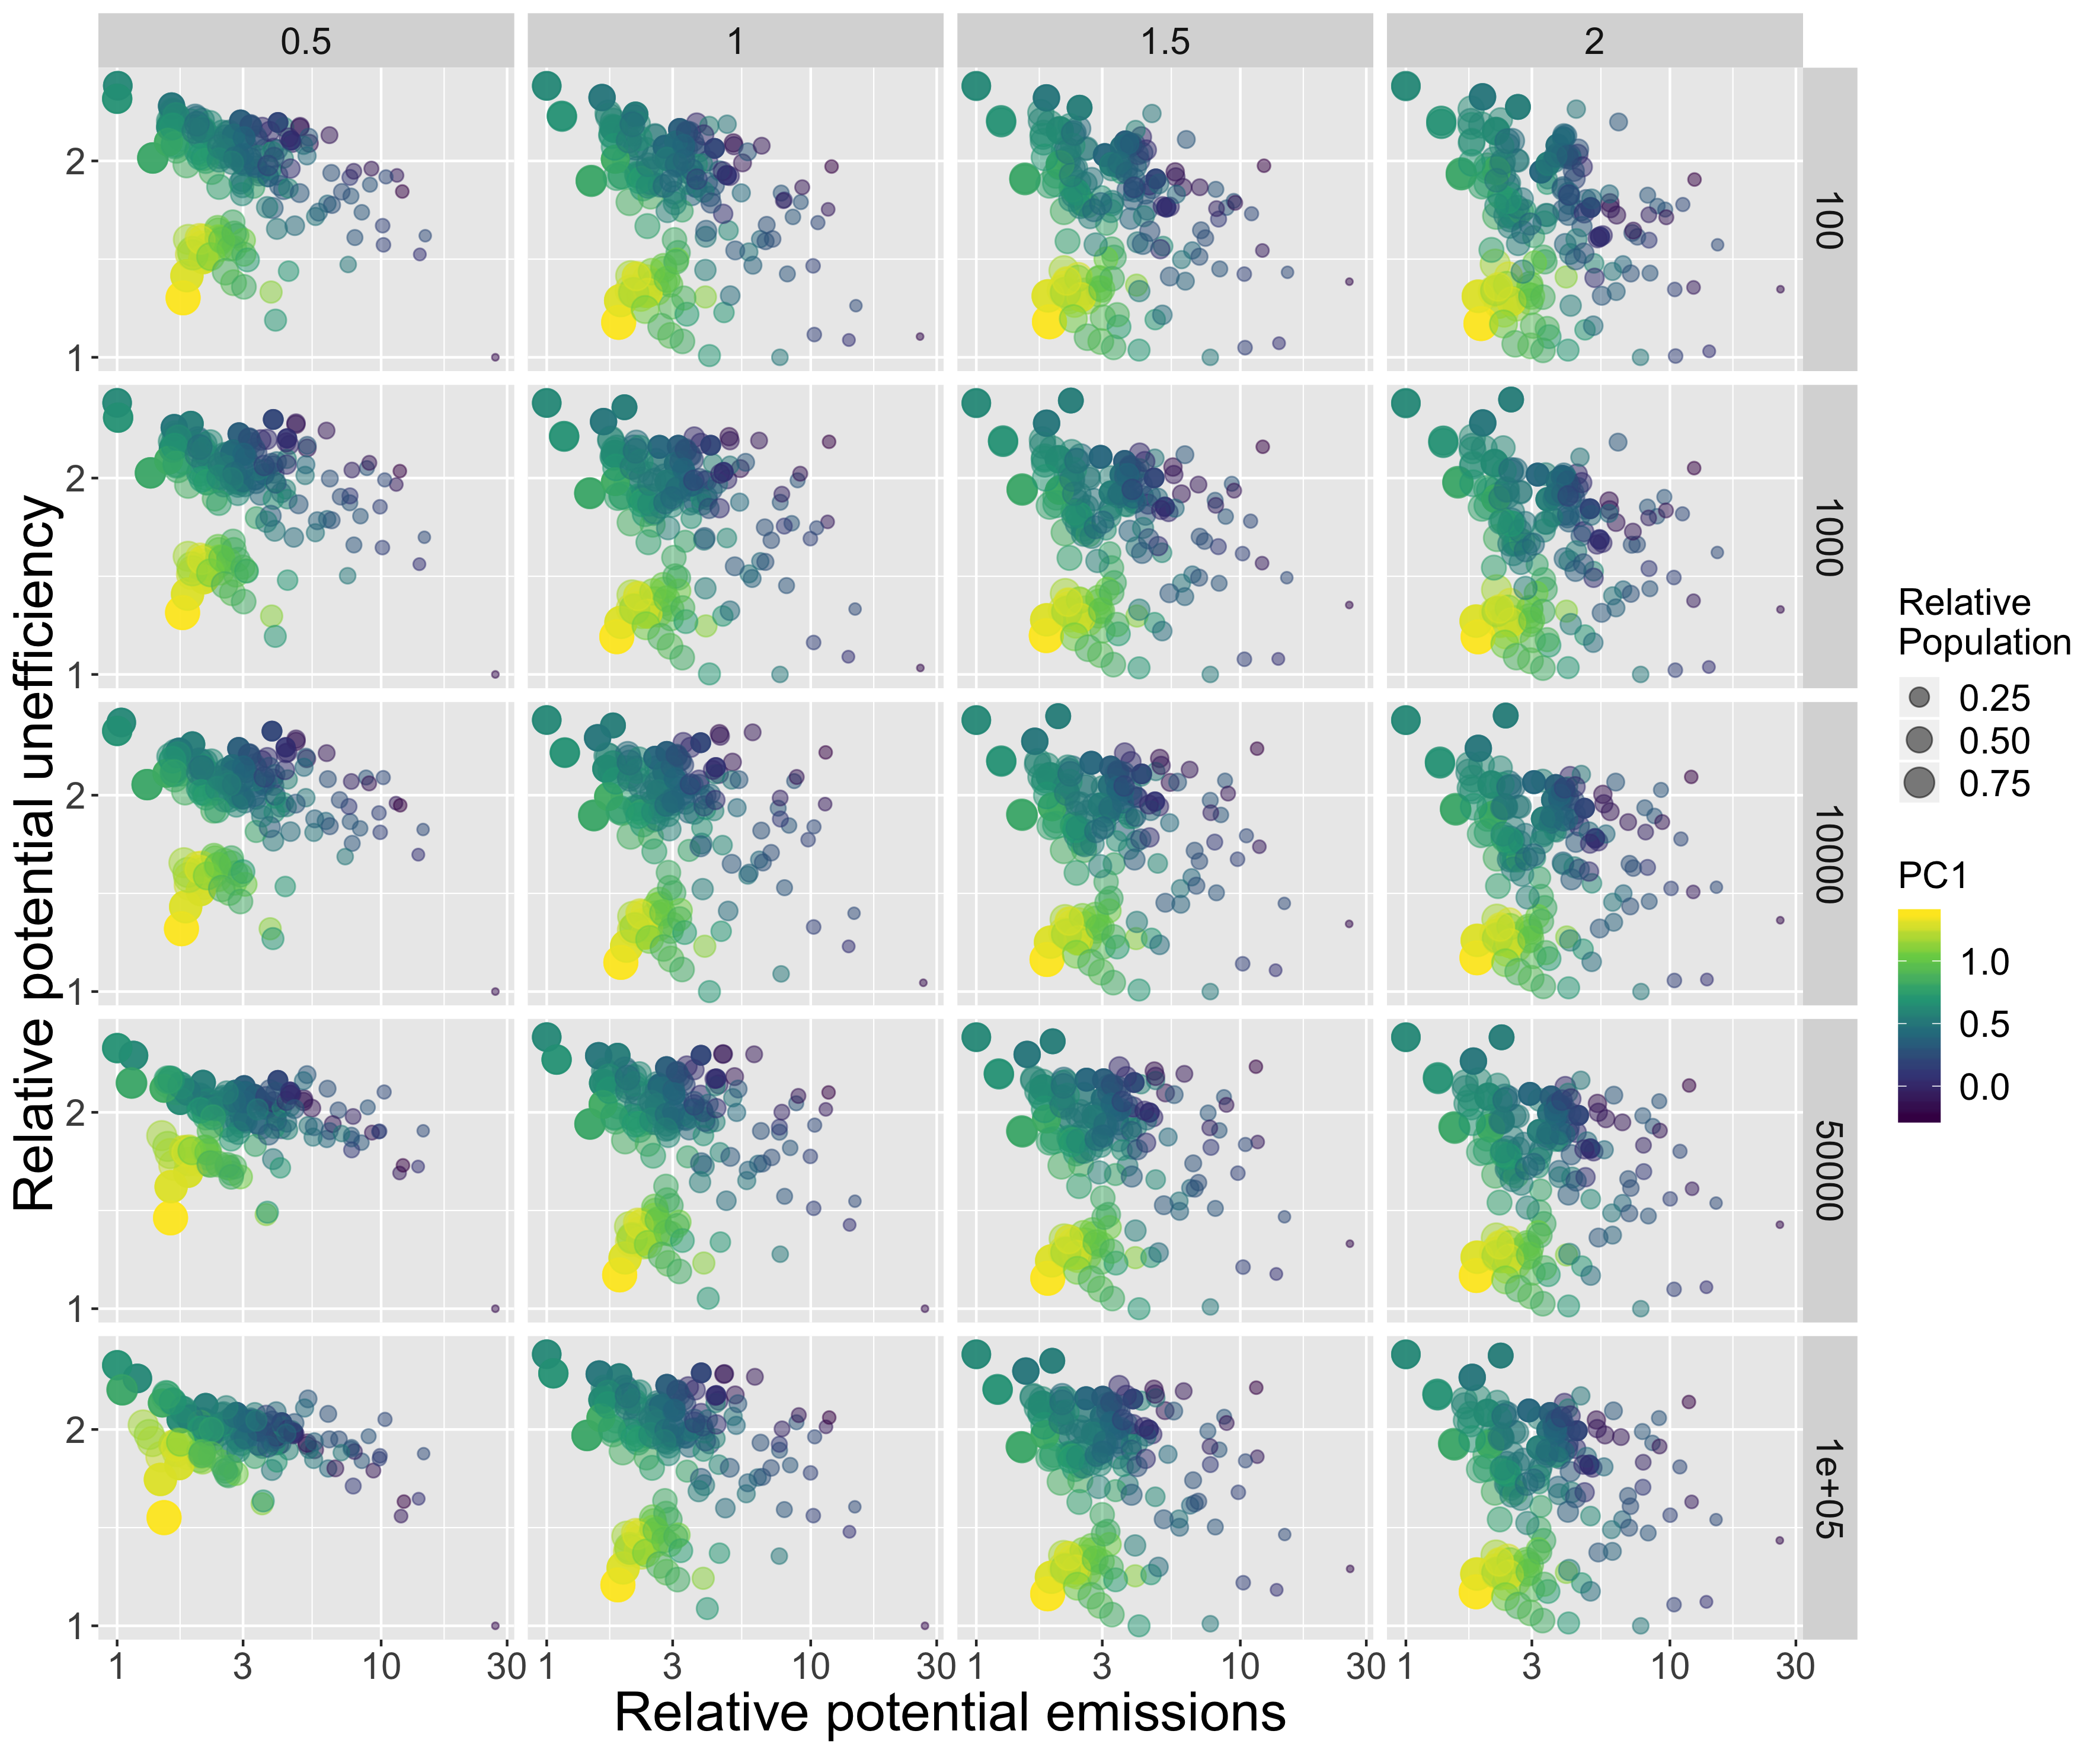
\includegraphics[width=0.49\textwidth]{figures/aggreg_morpho_relemissions-relefficiency_colpc1_logscale.png}
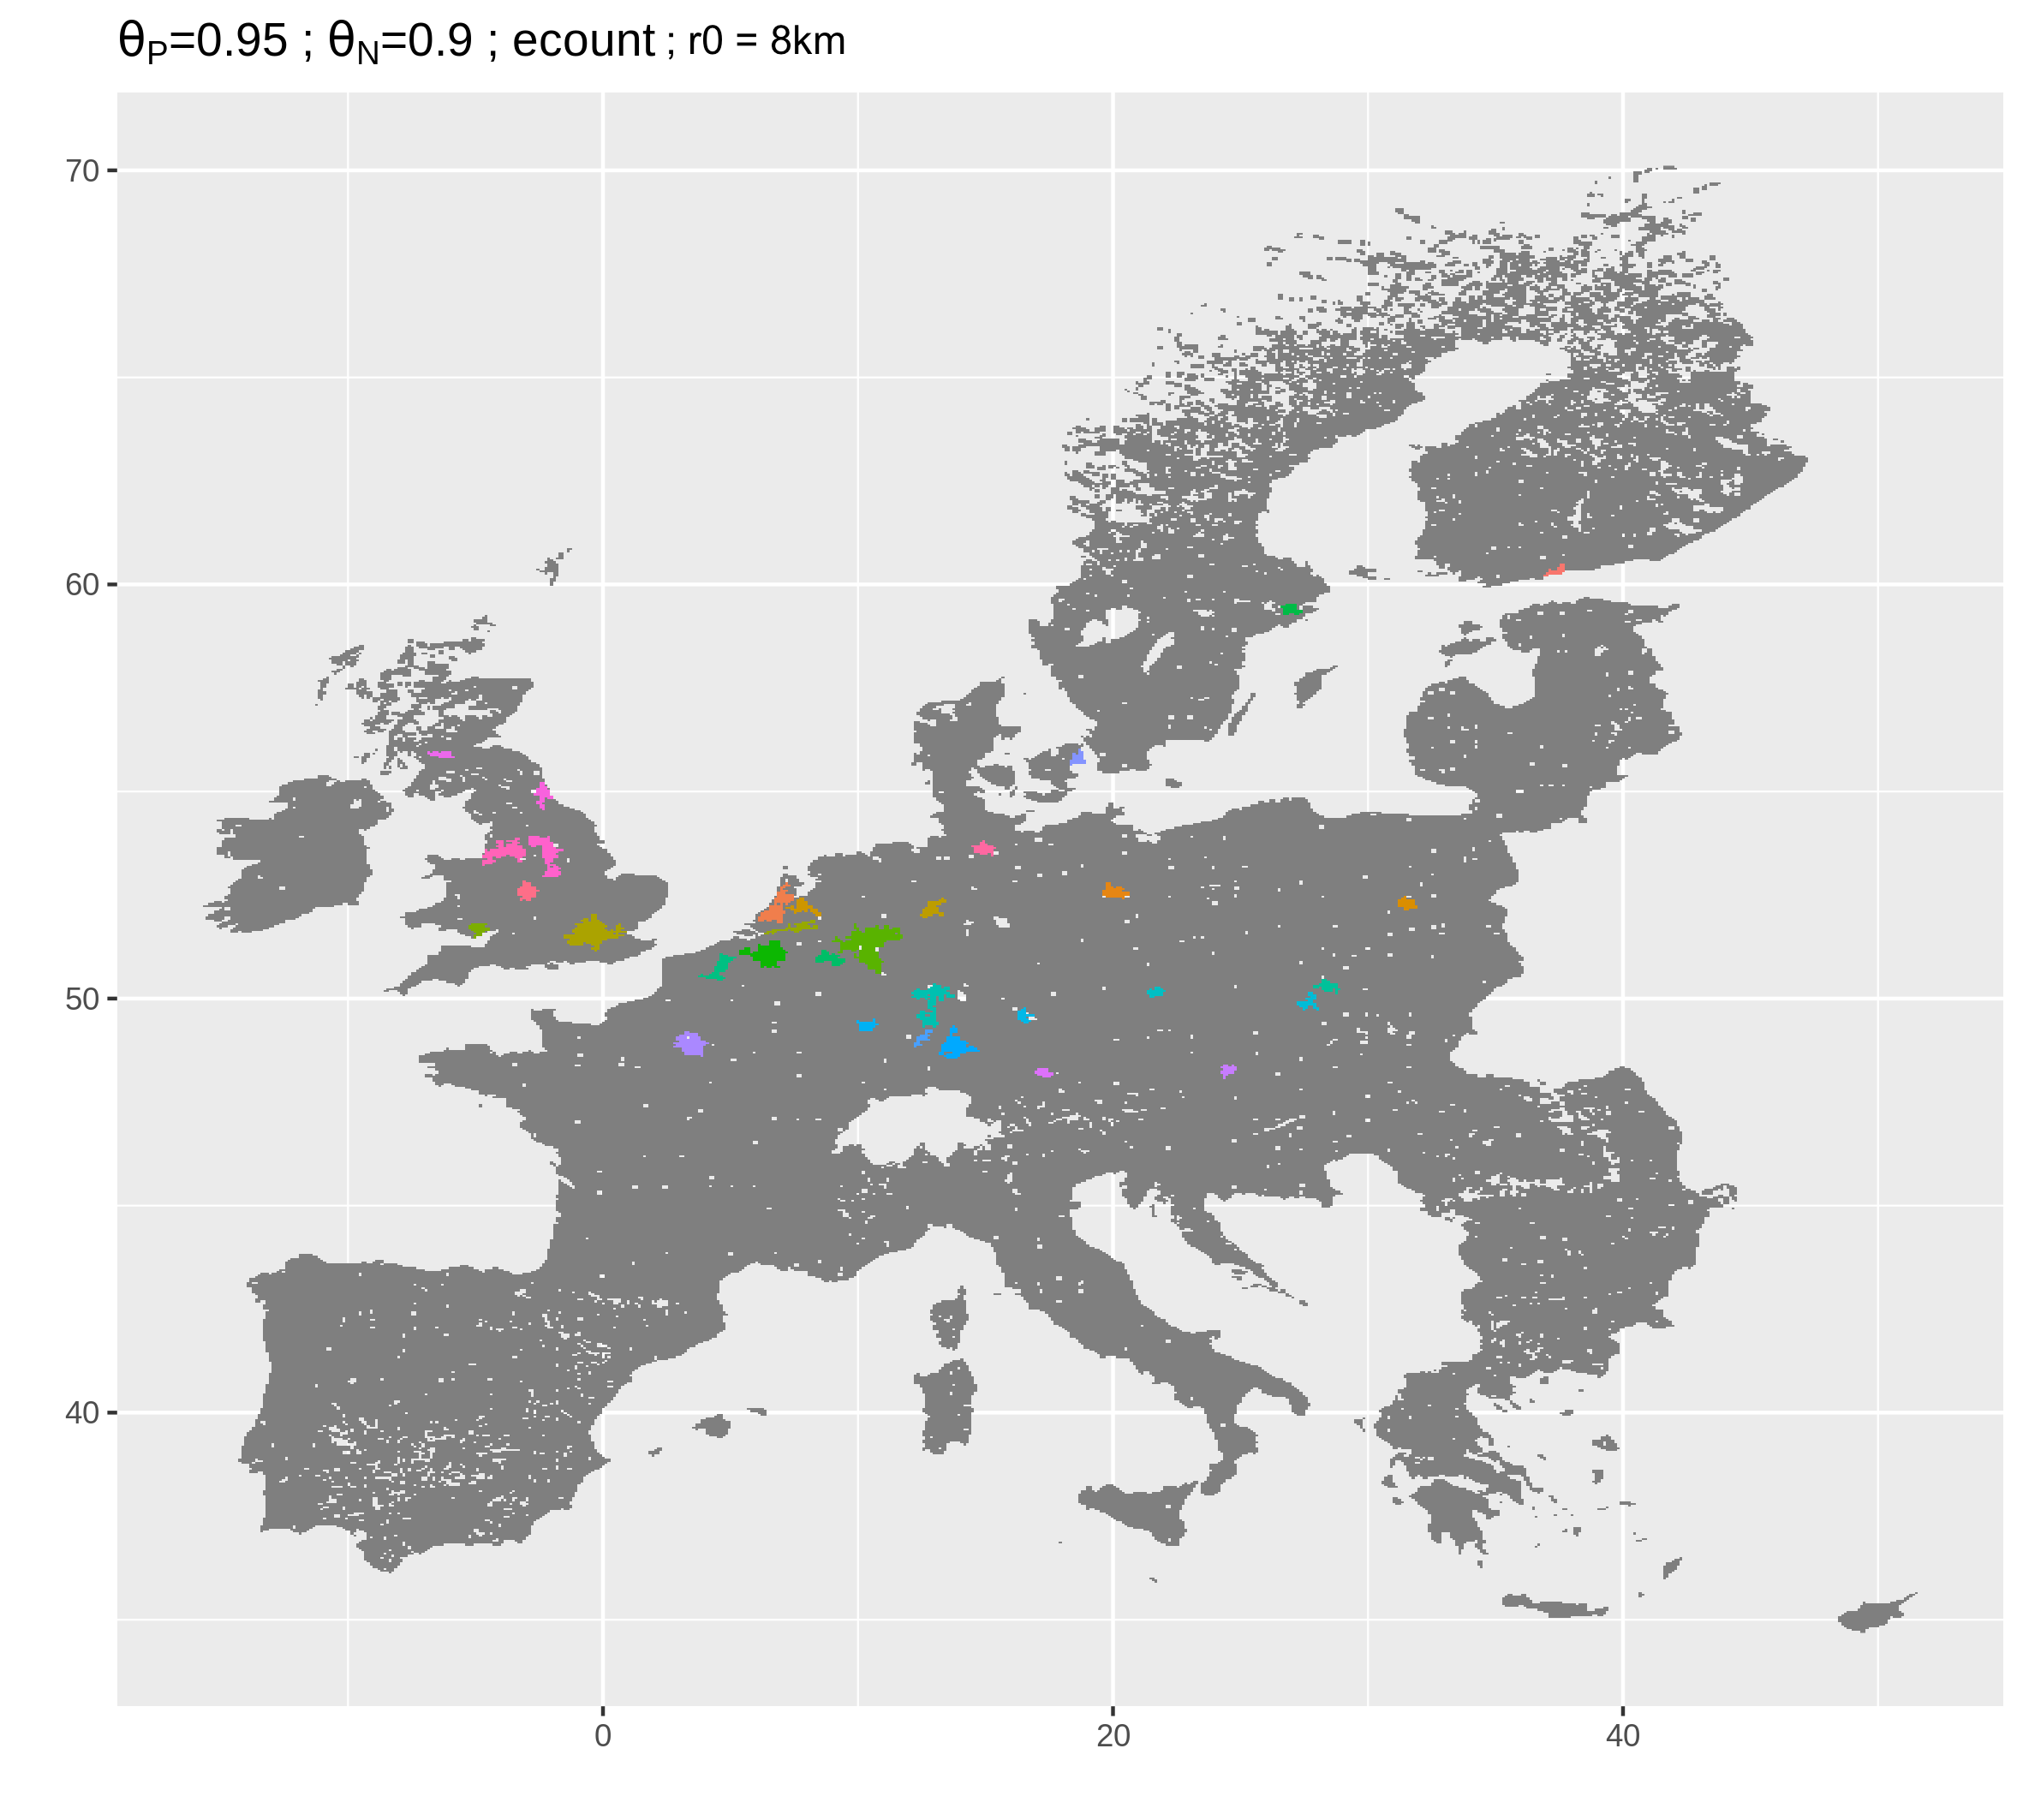
\includegraphics[width=0.49\textwidth]{figures/totalPop4183694_00056402_ecount850_radius8000.png}

\tiny

\bigskip

Raimbault, J. (2019). Multi-dimensional Urban Network Percolation. arXiv preprint arXiv:1903.07141.

}







\sframe{Conclusion}{

\justify

$\rightarrow$ Multiple ways to model urban systems: \textbf{towards more interdisciplinary coupling and comparison of models.}

\smallskip

$\rightarrow$ At which scale? \textbf{Towards multi-scale models.}

\smallskip

$\rightarrow$ With complementary aspects of knowledge? \textbf{Need for knowledge domain integration.}


\bigskip

\textbf{To use OpenMOLE (free and open software) and contribute: }\\
\url{next.openmole.org}

\bigskip


%
\textbf{Some references}

\medskip

\tiny

%
%
%\medskip


%Raimbault, J. (2018). Caract{\'e}risation et mod{\'e}lisation de la co-{\'e}volution des r{\'e}seaux de transport et des territoires (Doctoral dissertation, Université Paris 7 Denis Diderot). \url{https://halshs.archives-ouvertes.fr/tel-01857741}

Raimbault, J. (2017). An Applied Knowledge Framework to Study Complex Systems. In Complex Systems Design \& Management (pp. 31-45). arXiv:1706.09244.

\smallskip

Raimbault, J. (2018). Indirect evidence of network effects in a system of cities. Environment and Planning B: Urban Analytics and City Science, 2399808318774335.

\smallskip

Raimbault, J. (2018). Calibration of a density-based model of urban morphogenesis. PloS one, 13(9), e0203516.

\smallskip

Raimbault, J. (2019). An urban morphogenesis model capturing interactions between networks and territories. In The Mathematics of Urban Morphology (pp. 383-409). Birkhäuser, Cham.

\smallskip

Raimbault, J. (2019). Modeling the co-evolution of cities and networks. In Niel, Z., Rozenblat, C., eds. \textit{Handbook of Cities and Networks}, Edwar Elgar Publishing, \textit{in press}. arXiv:1804.09430



%
%
%
%
%%\smallskip
%
%%\textbf{Open repository} at \texttt{https://github.com/JusteRaimbault/UrbanGrowth}\\\smallskip
%%\textbf{Acknowledgments}: thanks to the \textit{EGI} for access to the infrastructure.
%
%
}
%
%

\sframe{Submit to special session at CCS}{


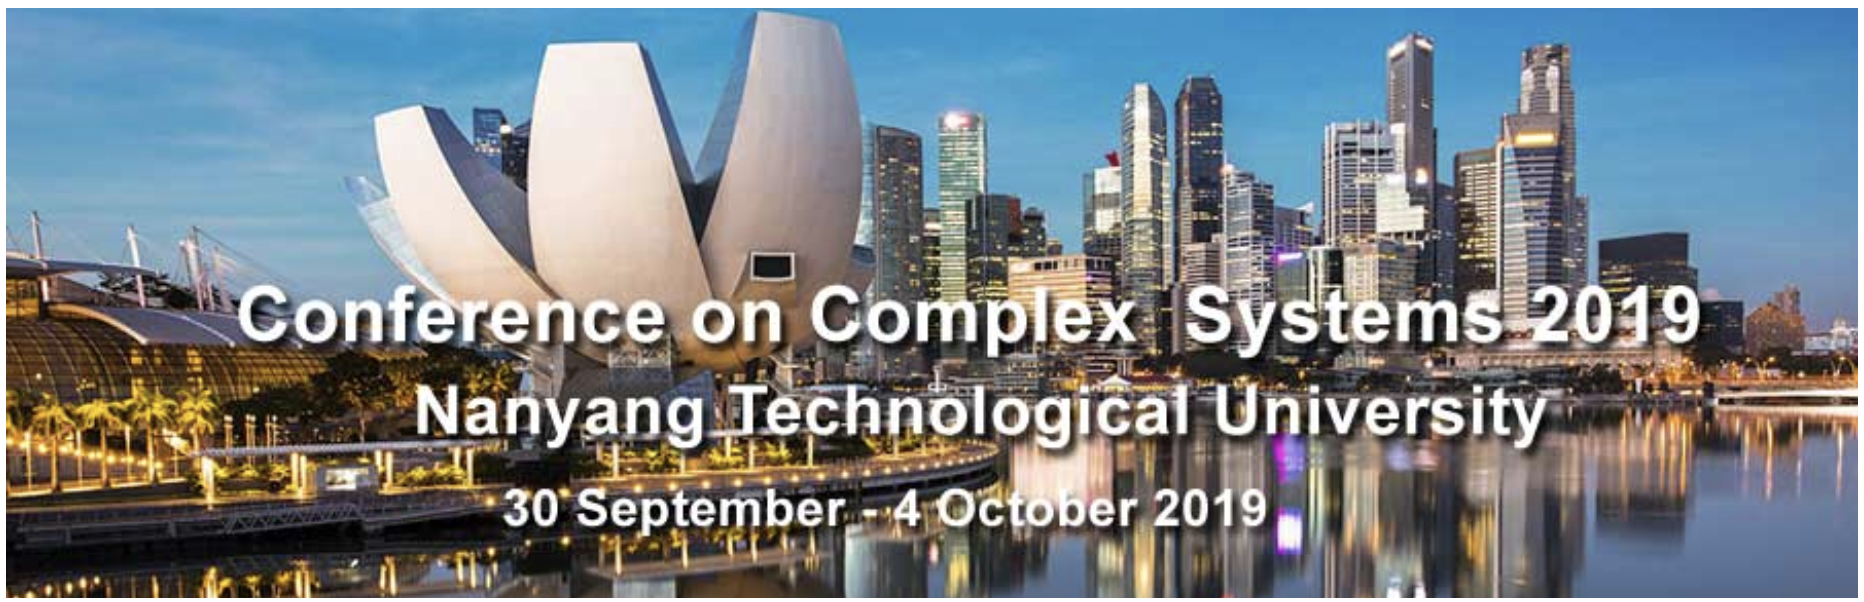
\includegraphics[width=\linewidth]{figures/ccs.png}

\medskip

\textit{Satellite session on methods and epistemology in modeling and simulation, at Conference on Complex Systems, 2nd October 2019}

\smallskip

\textbf{Submit your abstract before July 7th!}

\url{https://iscpif.fr/ccs-satelllite-session-2019-new-methods/}

\smallskip

\textbf{Submission link:}

\url{https://easychair.org/conferences/?conf=simexplo2019}

}




%%%%%%%%%%%%%%%%%%%%%
\begin{frame}[allowframebreaks]
\frametitle{References}
\bibliographystyle{apalike}
\bibliography{/Users/juste/ComplexSystems/CityNetwork/Biblio/Bibtex/CityNetwork,biblio}
\end{frame}
%%%%%%%%%%%%%%%%%%%%%%%%%%%%










\end{document}















